\ifdefined\maindoc
% Under the thesis build, main.tex owns the full \graphicspath list. \graphicspath REPLACES
% rather than appends, so this branch deliberately does nothing.
\else
\documentclass[12pt]{report}
\usepackage[a4paper,margin=1in]{geometry}
\usepackage[utf8]{inputenc}
\usepackage[T1]{fontenc}
\usepackage[british]{babel}
\usepackage{amsmath,amssymb,amsthm}
\usepackage{booktabs}
\usepackage{setspace}
\usepackage{graphicx}
\usepackage{subcaption}
\usepackage{enumitem}
\usepackage{threeparttable}
\usepackage{placeins}
\usepackage{longtable}
\usepackage{hyperref}
\usepackage{array}
\usepackage{pdflscape}
\usepackage{makecell}
\usepackage{algorithm}
\usepackage{algpseudocode}
\newcommand{\STATE}{\State}
\newcommand{\COMMENT}[1]{\Comment{#1}}
\newcommand{\RETURN}{\State \textbf{return} }
\newcommand{\IF}[1]{\If{#1}}
\newcommand{\ELSE}{\Else}
\newcommand{\ENDIF}{\EndIf}
\newcommand{\FOR}[1]{\For{#1}}
\newcommand{\ENDFOR}{\EndFor}
\newcommand{\WHILE}[1]{\While{#1}}
\newcommand{\ENDWHILE}{\EndWhile}
\usepackage[backend=biber,style=ieee,citestyle=numeric-comp,sorting=none]{biblatex}
\addbibresource{../../references.bib}
\newtheorem{proposition}{Proposition}
\newtheorem{definition}{Definition}
\onehalfspacing
\graphicspath{{figures/}}
% Standalone-only fallbacks. Numbering: 1 Introduction, 2 Background, 3 Network Model,
% 4 Network Decomposition, 5 Probability, 6 this chapter, 7 Critical Path, 8 Julia package,
% 9 Interface, 10 Integrated Case Study, 11 Conclusions.
\makeatletter
\newlabel{ch:lit-review}{{2}{1}{}{Doc-Start}{}}
\newlabel{ch:system-model}{{3}{1}{}{Doc-Start}{}}
\newlabel{ch:diamond-module}{{4}{1}{}{Doc-Start}{}}
\newlabel{ch:probability-toolkit}{{5}{1}{}{Doc-Start}{}}
\newlabel{ch:critical-path}{{7}{1}{}{Doc-Start}{}}
\newlabel{ch:julia-package}{{8}{1}{}{Doc-Start}{}}
\newlabel{ch:front-end}{{9}{1}{}{Doc-Start}{}}
\newlabel{ch:integrated-case-study}{{10}{1}{}{Doc-Start}{}}
\newlabel{ch:conclusions}{{11}{1}{}{Doc-Start}{}}
\newlabel{app:network-specs}{{A}{1}{}{Doc-Start}{}}
\newlabel{app:full-results}{{B}{1}{}{Doc-Start}{}}
\makeatother
\begin{document}
\title{Information as Resources: Capacity Flow Toolkit}
\fi

\providecommand{\PH}[1]{\textbf{[#1]}}

\section{Introduction}
\label{sec:flow-intro}

A network that is connected can still fail to deliver. When a pipe is throttled, a feeder is
derated or a treatment stage is running below its design rate, supply reaches every demand
point and the amount that arrives is short of what is needed. The probabilistic
interpretation of Chapter~\ref{ch:probability-toolkit} asks whether supply reaches a node;
the capacity interpretation asks how much, and what limits it. Under this interpretation the
value attached to an edge is the most that can pass along it and the value attached to a
node is the most that can pass through it. The Capacity Flow Toolkit is the set of modules
that answers the second question. It reads the graph object of Chapter~\ref{ch:system-model}
directly, uses neither the layered iteration sets nor the Network Decomposition Module of
Chapter~\ref{ch:diamond-module}, and is point-valued: every capacity is a single number,
and no interval or probability-box propagation is claimed for this interpretation. Built on
the maximum-flow minimum-cut theory reviewed in Chapter~\ref{ch:lit-review}, the toolkit
answers six questions about a capacitated DAG:

\begin{enumerate}[label=\textbf{Q\arabic*.}]
    \item What maximum throughput can the network deliver under its current capacities?
    \item Which cut sets form the binding bottleneck on that throughput, and how many
      equivalent cuts are there?
    \item Which component failures or capacity reductions most reduce deliverable flow?
    \item What capacity change on a given edge maintains, or first reaches, a target service
      level?
    \item How much path-disjoint redundancy exists between sources and sinks?
    \item Which components are single points of failure?
\end{enumerate}

What is new in this chapter is the collection of these answers on one graph object, with
every one of them checked. The flow model is stated with its reductions for several sources
and sinks and for node capacities, each proved exact (Section~\ref{sec:flow-model}). Three
maximum-flow solvers are provided, with post-solve checks on every result
(Section~\ref{sec:flow-solvers}). The six questions are answered by modules that share one
baseline solve, among them an enumeration of every minimum cut through the residual lattice,
failure analyses over brute-force and candidate-restricted sets, and a parametric threshold
method that uses the piecewise-linear dependence of the maximum flow on a single capacity
(Sections~\ref{sec:flow-questions} and~\ref{sec:flow-cost}). Every module is validated
against an independent computation on a corpus of twelve networks and on generated
instances of up to $10^5$ edges (Section~\ref{sec:flow-validation}), and the toolkit is
applied to the IEEE Reliability Test System (Section~\ref{sec:flow-cases}). The chapter
closes with the limitations of a point-valued flow model and the extensions that follow from
it. Section~\ref{sec:flow-background} first recalls what the chapter builds on.

\section{Background}
\label{sec:flow-background}

Chapter~\ref{ch:lit-review} reviewed the maximum-flow minimum-cut theorem of Ford and
Fulkerson \cite{ford1956,ford1962} and three results from the same theory that this toolkit
uses. A node with its own capacity is handled by splitting it into an entry node and an exit
node joined by an edge of that capacity. Any feasible flow decomposes into source-to-sink
path flows that sum to the total. The minimum cuts of a network lie between the set of nodes
reachable from the source in the residual graph and the set that can reach the sink in the
reverse residual graph. Menger's theorem, in its edge and node
forms, gives the number of disjoint paths as a unit-capacity maximum flow. The Birnbaum
importance of a component \cite{birnbaum1969} is the model for the marginal measures of
Section~\ref{sec:flow-sensitivity}, with the difference that here it is a throughput range
without a probability weighting.

Chapter~\ref{ch:lit-review} also reviewed the two treatments of uncertain capacities in the
literature, the adversarial uncertainty set of robust optimisation
\cite{bertsimas2013robust} and the discrete random capacity of stochastic-flow reliability
\cite{doulliez1972transportation}. Neither is implemented here. The toolkit computes exact
answers for a single point-valued capacity assignment, and a best-case and worst-case pair of
assignments is two separate solves.

\section{The Flow Model}
\label{sec:flow-model}
Let
\[
G=(V,E)
\]
be a directed acyclic graph with edge-capacity function
\[
c:E\to\mathbb{R}_{\ge 0},
\]
where \(c_{uv}\) is the maximum admissible flow on edge \((u,v)\in E\). When node capacities are modelled, let
\[
b:V\to\mathbb{R}_{\ge 0}.
\]
Here \(b_v\) denotes the maximum admissible through-flow at node \(v\).
Define the flow variable
\[
f:E\to\mathbb{R}_{\ge 0},
\]
with \(f_{uv}:=f((u,v))\) for each edge \((u,v)\in E\).
For node \(v\), define
\[
\delta^+(v):=\{(v,w)\in E\}, \qquad \delta^-(v):=\{(u,v)\in E\}
\]
as the outgoing and incoming edge sets, respectively. For a capacitated network model \(G\) with designated source and sink nodes \(s,t\in V\), the primary objective is to compute the maximum deliverable throughput from \(s\) to \(t\), subject to edge capacities \(c_{uv}\) for \((u,v)\in E\) and, when modelled, node through-flow bounds \(b_v\) for \(v\in V\).


First consider a base-case network: a single-source single-sink capacitated DAG, shown in Fig.~\ref{fig:toy_siso_symbolic}. Node \(s\) is the source, node \(t\) is the sink, and intermediate nodes relay flow under capacity constraints. The performance measure is the deliverable throughput from \(s\) to \(t\), a finer quantity than simple path connectivity.

\begin{figure}[ht]
\centering
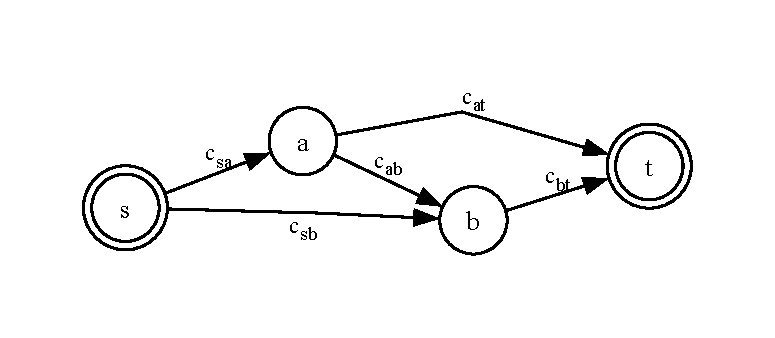
\includegraphics[width=0.70\textwidth]{toy_siso_symbolic.pdf}
\caption{Minimal single-source single-sink capacitated DAG network.}
\label{fig:toy_siso_symbolic}
\end{figure}

For this base case, let \(f:E\to\mathbb{R}_{\ge 0}\) and \(F\in\mathbb{R}_{\ge 0}\) be decision variables, where \(F\) is the total delivered flow from \(s\) to \(t\). The optimisation model is
\[
\max\; F
\]
subject to
\begin{align}
0 \le f_{uv} \le c_{uv}, &\qquad \forall (u,v)\in E, \label{eq:cap}\\
\sum_{e\in\delta^-(v)} f_e - \sum_{e\in\delta^+(v)} f_e &= 0,
\qquad \forall v\in V\setminus\{s,t\}, \label{eq:cons}\\
\sum_{e\in\delta^+(s)} f_e - \sum_{e\in\delta^-(s)} f_e &= F, \label{eq:source}\\
\sum_{e\in\delta^-(t)} f_e - \sum_{e\in\delta^+(t)} f_e &= F. \label{eq:sink}
\end{align}

Taking \(F^\star\) as the optimal (maximum feasible) value of \(F\), if the sink node \(t\) has a required demand level \(D_t\), the flow module quantifies service adequacy through the throughput margin
\[
\Delta_t := F^\star - D_t,
\]
where \(\Delta_t\ge 0\) means that the network can meet demand with residual margin, and \(\Delta_t<0\) indicates a throughput shortfall of \(|\Delta_t|\).



\subsection{Several sources and sinks}
Let the source set be \(S\subseteq V\) and the sink set be \(T\subseteq V\), with \(|S|\ge 1\) and \(|T|\ge 1\). Figure~\ref{fig:msss_reduction}a shows the original multi-source multi-sink network.

By introducing a super-source \(s^\star\) and a super-sink \(t^\star\), as shown in Fig.~\ref{fig:msss_reduction}b, the reduced graph is
\[
V' = V\cup\{s^\star,t^\star\},
\]
\[
E' = E \cup \{(s^\star,s): s\in S\} \cup \{(t,t^\star): t\in T\}.
\]
The connector capacities are set to non-binding values (implemented as \(\mathrm{Inf}\) in the solver):
\[
c_{s^\star s}=+\infty\ \forall s\in S, \qquad c_{t t^\star}=+\infty\ \forall t\in T.
\]

\begin{figure}[ht]
\centering
\begin{subfigure}[t]{0.47\textwidth}
\centering
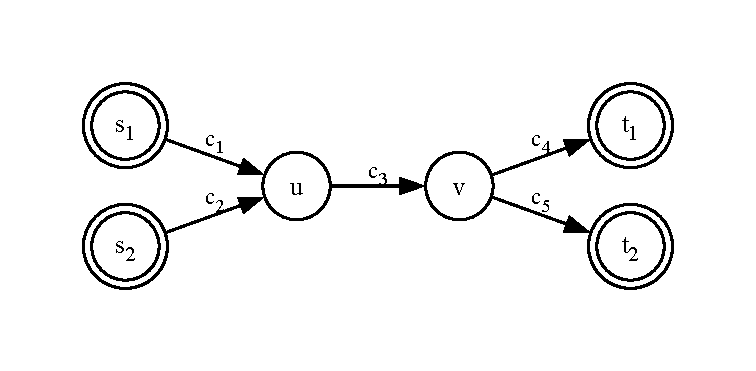
\includegraphics[width=\textwidth]{msss_original.pdf}
\caption{Original multi-source multi-sink network.}
\end{subfigure}
\hfill
\begin{subfigure}[t]{0.47\textwidth}
\centering
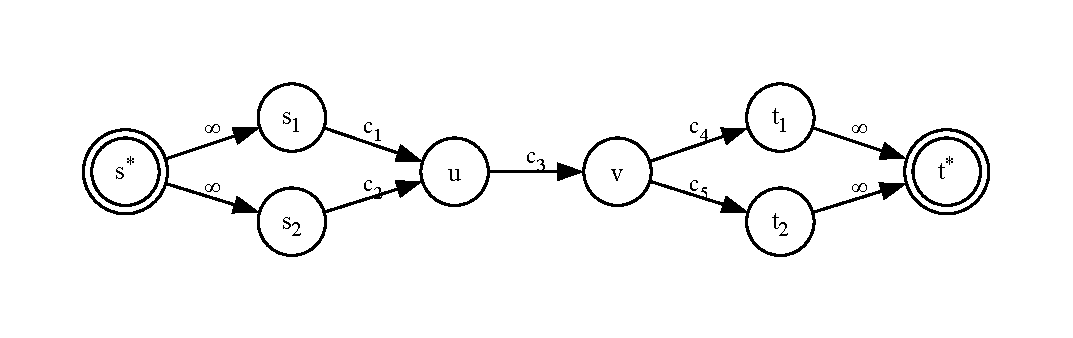
\includegraphics[width=\textwidth]{msss_super_reduction.pdf}
\caption{Equivalent super-source/super-sink reduction.}
\end{subfigure}
\caption{Graph reduction of a multi-source multi-sink capacitated DAG to an equivalent single-source single-sink max-flow problem.}
\label{fig:msss_reduction}
\end{figure}

\begin{proposition}[Exactness of the super-terminal reduction]
The optimal value of the multi-source multi-sink max-flow problem on \(G\) is equal to the optimal value of the single-source single-sink max-flow problem on the reduced graph \(G'=(V',E')\) with terminals \(s^\star\) and \(t^\star\).
\end{proposition}

\begin{proof}
Let \(f\) be any feasible flow for the original multi-terminal problem with total value \(F\).

We may define an augmented flow \(f'\) on \(G'\) by retaining the values of \(f\) on all original edges, setting
\[
f'_{s^\star s}:=\sum_{e\in\delta^+(s)} f_e - \sum_{e\in\delta^-(s)} f_e \qquad \forall s\in S,
\]
and
\[
f'_{t t^\star}:=\sum_{e\in\delta^-(t)} f_e - \sum_{e\in\delta^+(t)} f_e \qquad \forall t\in T.
\]
Since the connector edges are guaranteed to be non-binding, all capacity constraints from the original network remain satisfied. Naturally, flow conservation holds at every original transit node, while the net outflow from \(s^\star\) and the net inflow to \(t^\star\) are both equal to \(F\). Therefore \(f'\) is a feasible \(s^\star\)-\(t^\star\) flow of value \(F\).

Conversely, let \(f'\) be any feasible \(s^\star\)-\(t^\star\) flow on \(G'\): then, restricting \(f'\) to the original edge set \(E\) gives a flow \(f\) on \(G\). Again, conservation on all nodes in \(V\setminus(S\cup T)\) is inherited directly from the reduced problem, and the super-terminal connectors account exactly for aggregate injection at the sources and aggregate withdrawal at the sinks. Therefore \(f\) is feasible for the original multi-terminal problem and has the same total value as \(f'\). Since feasible flows map in both directions without changing objective value, the two optimal values are equal.
\end{proof}

Thus, solving the reduced super-source/super-sink problem is equivalent to solving the original multi-terminal problem, which is:
\[
\max\; F
\]
subject to
\begin{align}
0 \le f_{uv} \le c_{uv}, &\qquad \forall (u,v)\in E, \\
\sum_{e\in\delta^-(v)} f_e - \sum_{e\in\delta^+(v)} f_e &= 0,
\qquad \forall v\in V\setminus(S\cup T), \label{eq:msss-transit}\\
\sum_{s\in S}\left(\sum_{e\in\delta^+(s)} f_e - \sum_{e\in\delta^-(s)} f_e\right) &= F, \label{eq:msss-source}\\
\sum_{t\in T}\left(\sum_{e\in\delta^-(t)} f_e - \sum_{e\in\delta^+(t)} f_e\right) &= F. \label{eq:msss-sink}
\end{align}


\subsection{Node capacities by node splitting}
\label{sec:node_splitting}

The framework accepts values on nodes as well as on edges, so a through-flow limit on a component can be modelled directly.
As shown in Figure~\ref{fig:nodecap_reduction}, this work adopts a node-splitting approach where each constrained node \(v\in V_c\) is replaced by an input node \(v^-\) and an output node \(v^+\), connected by an internal edge:
\[
(v^{-},v^{+}), \qquad c_{v^{-}v^{+}}=b_v.
\]
The original incoming edges of \(v\) are redirected to \(v^-\), and every original outgoing edge is emitted from \(v^+\).

\begin{figure}[ht]
\centering
\begin{subfigure}[t]{0.47\textwidth}
\centering
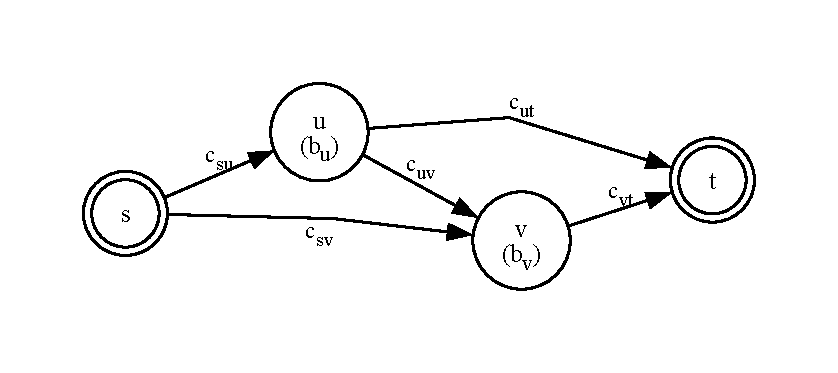
\includegraphics[width=\textwidth]{nodecap_original.pdf}
\caption{Original network with edge and node capacities.}
\end{subfigure}
\hfill
\begin{subfigure}[t]{0.47\textwidth}
\centering
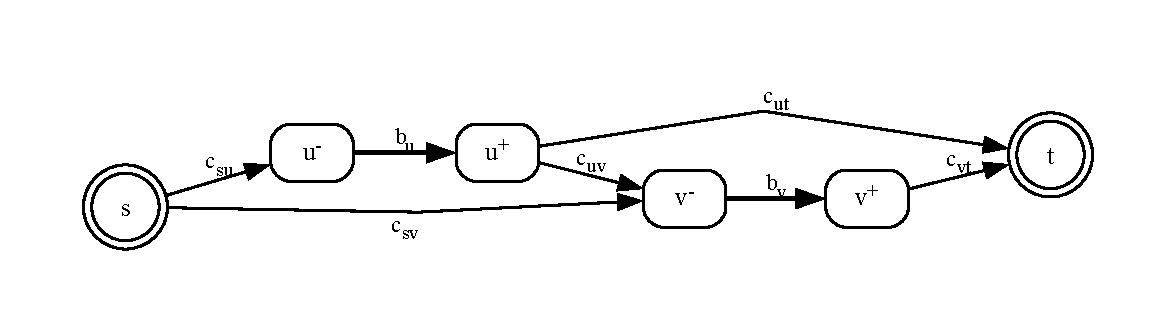
\includegraphics[width=\textwidth]{nodecap_split_equivalent.pdf}
\caption{Equivalent node-split edge-capacitated network.}
\end{subfigure}
\caption{Node-splitting transformation.}
\label{fig:nodecap_reduction}
\end{figure}


This extends the edge-capacitated flow model with 
\begin{align}
\sum_{e\in\delta^-(v)} f_e &\le b_v, \qquad \forall v\in V_c, \label{eq:nodecap-in}\\
\sum_{e\in\delta^+(v)} f_e &\le b_v, \qquad \forall v\in V_c. \label{eq:nodecap-out}
\end{align}
Here \(V_c\subseteq V\) may include source and sink nodes when terminal throughput limits are part of the model.

The optimisation model then becomes
\[
\max\; F
\]
subject to
\begin{align}
0 \le f_{uv} \le c_{uv}, &\qquad \forall (u,v)\in E, \label{eq:edgecap-both}\\
\sum_{e\in\delta^-(v)} f_e - \sum_{e\in\delta^+(v)} f_e &= 0,
\qquad \forall v\in V\setminus\{s,t\}, \label{eq:cons-both}\\
\sum_{e\in\delta^-(v)} f_e &\le b_v,
\qquad \forall v\in V_c, \label{eq:nodecap-both-in}\\
\sum_{e\in\delta^+(v)} f_e &\le b_v,
\qquad \forall v\in V_c, \label{eq:nodecap-both-out}\\
\sum_{e\in\delta^+(s)} f_e - \sum_{e\in\delta^-(s)} f_e &= F, \label{eq:source-both}\\
\sum_{e\in\delta^-(t)} f_e - \sum_{e\in\delta^+(t)} f_e &= F. \label{eq:sink-both}
\end{align}

\clearpage

\section{Maximum-Flow Solvers}
\label{sec:flow-solvers}
The toolkit provides three solvers for $F^\star$, summarised in Table~\ref{tab:solver_comparison}; the algorithms are standard and are described in Ahuja, Magnanti and Orlin \cite{ahuja_network_2014}. All three read the graph object of Chapter~\ref{ch:system-model} directly, apply the super-terminal reduction of Section~\ref{sec:flow-model} when the network has more than one source or sink, and return the flow, the min-cut partition and the flow value. When node capacities are supplied the node-splitting transformation is applied before the solve and the results are mapped back to the original nodes and edges, so that edge flows, sink allocations and cut-side node sets are reported on the network as given.

\begin{table}[ht]
\centering
\begin{threeparttable}
\begin{tabular}{p{3cm} p{4.5cm} p{4.5cm}}
\toprule
\textbf{Solver} & \textbf{Complexity} & \textbf{Best Fit} \\
\midrule
\texttt{:edmonds\_karp} & $O(VE^2)$ & Small networks \\
\texttt{:dinic}         & $O(V^2E)$ & Larger layered networks \\
\texttt{:push\_relabel} & $O(V^2E)$--$O(V^3)$\tnote{a} & Dense, high fan-out networks \\
\bottomrule
\end{tabular}
\begin{tablenotes}
\footnotesize
\item[a] Upper bound depends on node selection strategy; this solver does not enforce a highest-label invariant.
\end{tablenotes}
\end{threeparttable}
\caption{The three maximum-flow solvers.}
\label{tab:solver_comparison}
\end{table}

\subsection{Augmenting-path solvers}

By the max-flow min-cut theorem of Ford and Fulkerson~\cite{ford1956,ford1962}, the maximum flow from $s$ to $t$ equals the smallest total capacity of any set of edges whose removal separates them. The augmenting-path solvers compute both at once.


\begin{definition}[Residual Graph]
Given a capacitated network $G=(V,E)$ with capacity function 
$c:E\to\mathbb{R}_{\ge 0}$ and a feasible flow $f$, the residual 
graph $G_f=(V,E_f)$ is defined over the same node set $V$ with 
residual edge set
\[
E_f = \{(u,v)\in E : c_{uv} - f_{uv} > 0\} 
      \cup \{(v,u) : (u,v)\in E,\, f_{uv} > 0\},
\]
where the residual capacity on each edge is given by
\[
r_{uv} = \begin{cases} c_{uv} - f_{uv} & (u,v)\in E 
\quad \text{(forward residual)},\\ 
f_{vu} & (v,u)\in E \quad \text{(backward residual).}\end{cases}
\]
A forward residual edge $(u,v)$ represents spare capacity on an original edge; a backward residual edge $(v,u)$ represents flow on $(u,v)$ that can be cancelled.
An augmenting path $P$ in $G_f$ is then a directed path from 
$s$ to $t$ along which $r_{uv}>0$ for every edge $(u,v)\in P$.
\end{definition}

\begin{algorithm}[h]
\caption{Ford-Fulkerson Min-Cut Max-Flow}
\label{alg:ff-minmax}
\begin{algorithmic}[1]
\STATE Initialise residual graph $G_f \gets G$ with zero flow on all edges
\WHILE{there exists an augmenting path $P$ from source $s$ to sink $t$ in $G_f$}
    \STATE $\Delta \gets \min_{e \in P} c_f(e)$ \COMMENT{Bottleneck capacity along $P$}
    \FOR{each edge $e = (u,v) \in P$}
        \STATE $f(u,v) \gets f(u,v) + \Delta$ \COMMENT{Push flow forward}
        \STATE $f(v,u) \gets f(v,u) - \Delta$ \COMMENT{Update reverse edge}
    \ENDFOR
    \STATE Update $G_f$ to reflect new residual capacities
\ENDWHILE
\STATE Let $A$ be the set of nodes reachable from $s$ in $G_f$
\STATE Min-cut $= \{(u,v) \mid u \in A,\; v \notin A\}$
\RETURN Max-flow value $|f|$, min-cut set $A$
\end{algorithmic}
\end{algorithm}


As Algorithm~\ref{alg:ff-minmax} shows, the augmenting-path solvers repeatedly find a path and push flow along it. Most of the execution time is spent in four lookups:

\begin{itemize}
\item Capacity on any edge $u$-$v$
\item Current flow on any edge $u$-$v$
\item Outgoing edges from any node $u$ for graph search expansion
and forward residual updates
\item Incoming edges to any node $u$ for backward residual updates
and inflow queries
\end{itemize}

The graph object from the input processing module already stores this information as
part of the network structure and therefore does not need to be
recomputed on every call. Both Ford-Fulkerson-based solvers use this lookup structure 
but differ at step 2 in how the augmenting path is found.

\paragraph{Edmonds-Karp.} 
The Edmonds-Karp solver \cite{edmonds_theoretical_1972} uses a repeated breadth-first search (BFS) to find the shortest augmenting path in the residual graph. However, since each iteration requires an explicit path reconstruction via a stored parent map, the per-iteration overhead is higher than the Dinic variant, and the $O(VE^2)$ bound makes it poorly suited for larger and denser networks. It is therefore best reserved for smaller networks where simplicity and interpretability are preferred over performance.

\paragraph{Dinic.} 
To avoid the one-path-at-a-time limitation of the Edmonds-Karp method, the Dinic solver alternates between level graph construction via BFS and a blocking-flow depth-first search. The level graph restricts traversal to edges $u \to v$ where $\text{level}[v] = \text{level}[u] + 1$, reducing the search space to a layered subgraph per phase. Furthermore, to avoid the $O(E)$ per-path rescanning cost of naive DFS, this variant uses a pointer cursor \texttt{ptr[u]} to track each node's position in its adjacency list, permanently skipping exhausted edges. 

The Dinic solver is the best fit for most hierarchical DAG networks and is the framework's default when no user-specified option is selected. However, on very dense graphs with $O(V^2)$ edges and high structural redundancy, the per-phase BFS reconstruction becomes costly, and the blocking flow DFS must still handle a larger fraction of edges despite the pointer optimisation. In these cases, the Push-Relabel solver is recommended, as it operates locally without global path searches.

\subsection{Push-Relabel Solver}
Unlike the two path-based solvers, the Push-Relabel (PR) variant does not search for augmenting paths at all. This solver works by resolving excess flow locally from an initialised pre-flow.
Here, instead of a residual graph per phase, a merged neighbourhood list is built once over the augmented network and shared across all push and relabel operations. The algorithm proceeds as follows:

\begin{algorithm}[h]
\caption{Push-Relabel Min-Cut Max-Flow}
\label{alg:pr-minmax}
\begin{algorithmic}[1]
\STATE $\text{height}[s^\star] \gets |V|$; \quad $\text{height}[v] \gets 0 \;\forall\, v \neq s^\star$
\STATE Push maximum admissible flow from $s^\star$ to all neighbours; initialise $\text{excess}[v]$
\WHILE{$\exists$ active node $u$ with $\text{excess}[u] > 0$}
    \IF{$\exists$ neighbour $v$ with $r(u,v) > 0$ and $\text{height}[u] = \text{height}[v] + 1$}
        \STATE $\delta \gets \min(\text{excess}[u],\, r(u,v))$
        \STATE Push $\delta$ units from $u$ to $v$; update $\text{excess}[u]$, $\text{excess}[v]$, $r(u,v)$, $r(v,u)$
    \ELSE
        \STATE $\text{height}[u] \gets 1 + \min_{v:\, r(u,v)>0} \text{height}[v]$ \COMMENT{Relabel}
    \ENDIF
\ENDWHILE
\STATE Traverse final flow state from $s^\star$ to identify min-cut partition
\RETURN Max-flow value $|f|$, min-cut set
\end{algorithmic}
\end{algorithm}



\FloatBarrier

\section{The Questions the Toolkit Answers}
\label{sec:flow-questions}
The six questions of Section~\ref{sec:flow-intro} are answered by modules that share the solvers of Section~\ref{sec:flow-solvers}. Figure~\ref{fig:flow_toolkit_workflow} shows how the modules are called from one baseline solve. This section takes the questions in turn; the throughput question is the baseline solve itself and the margin $\Delta_t$ of Section~\ref{sec:flow-model}.


\begin{figure}[ht]
\centering
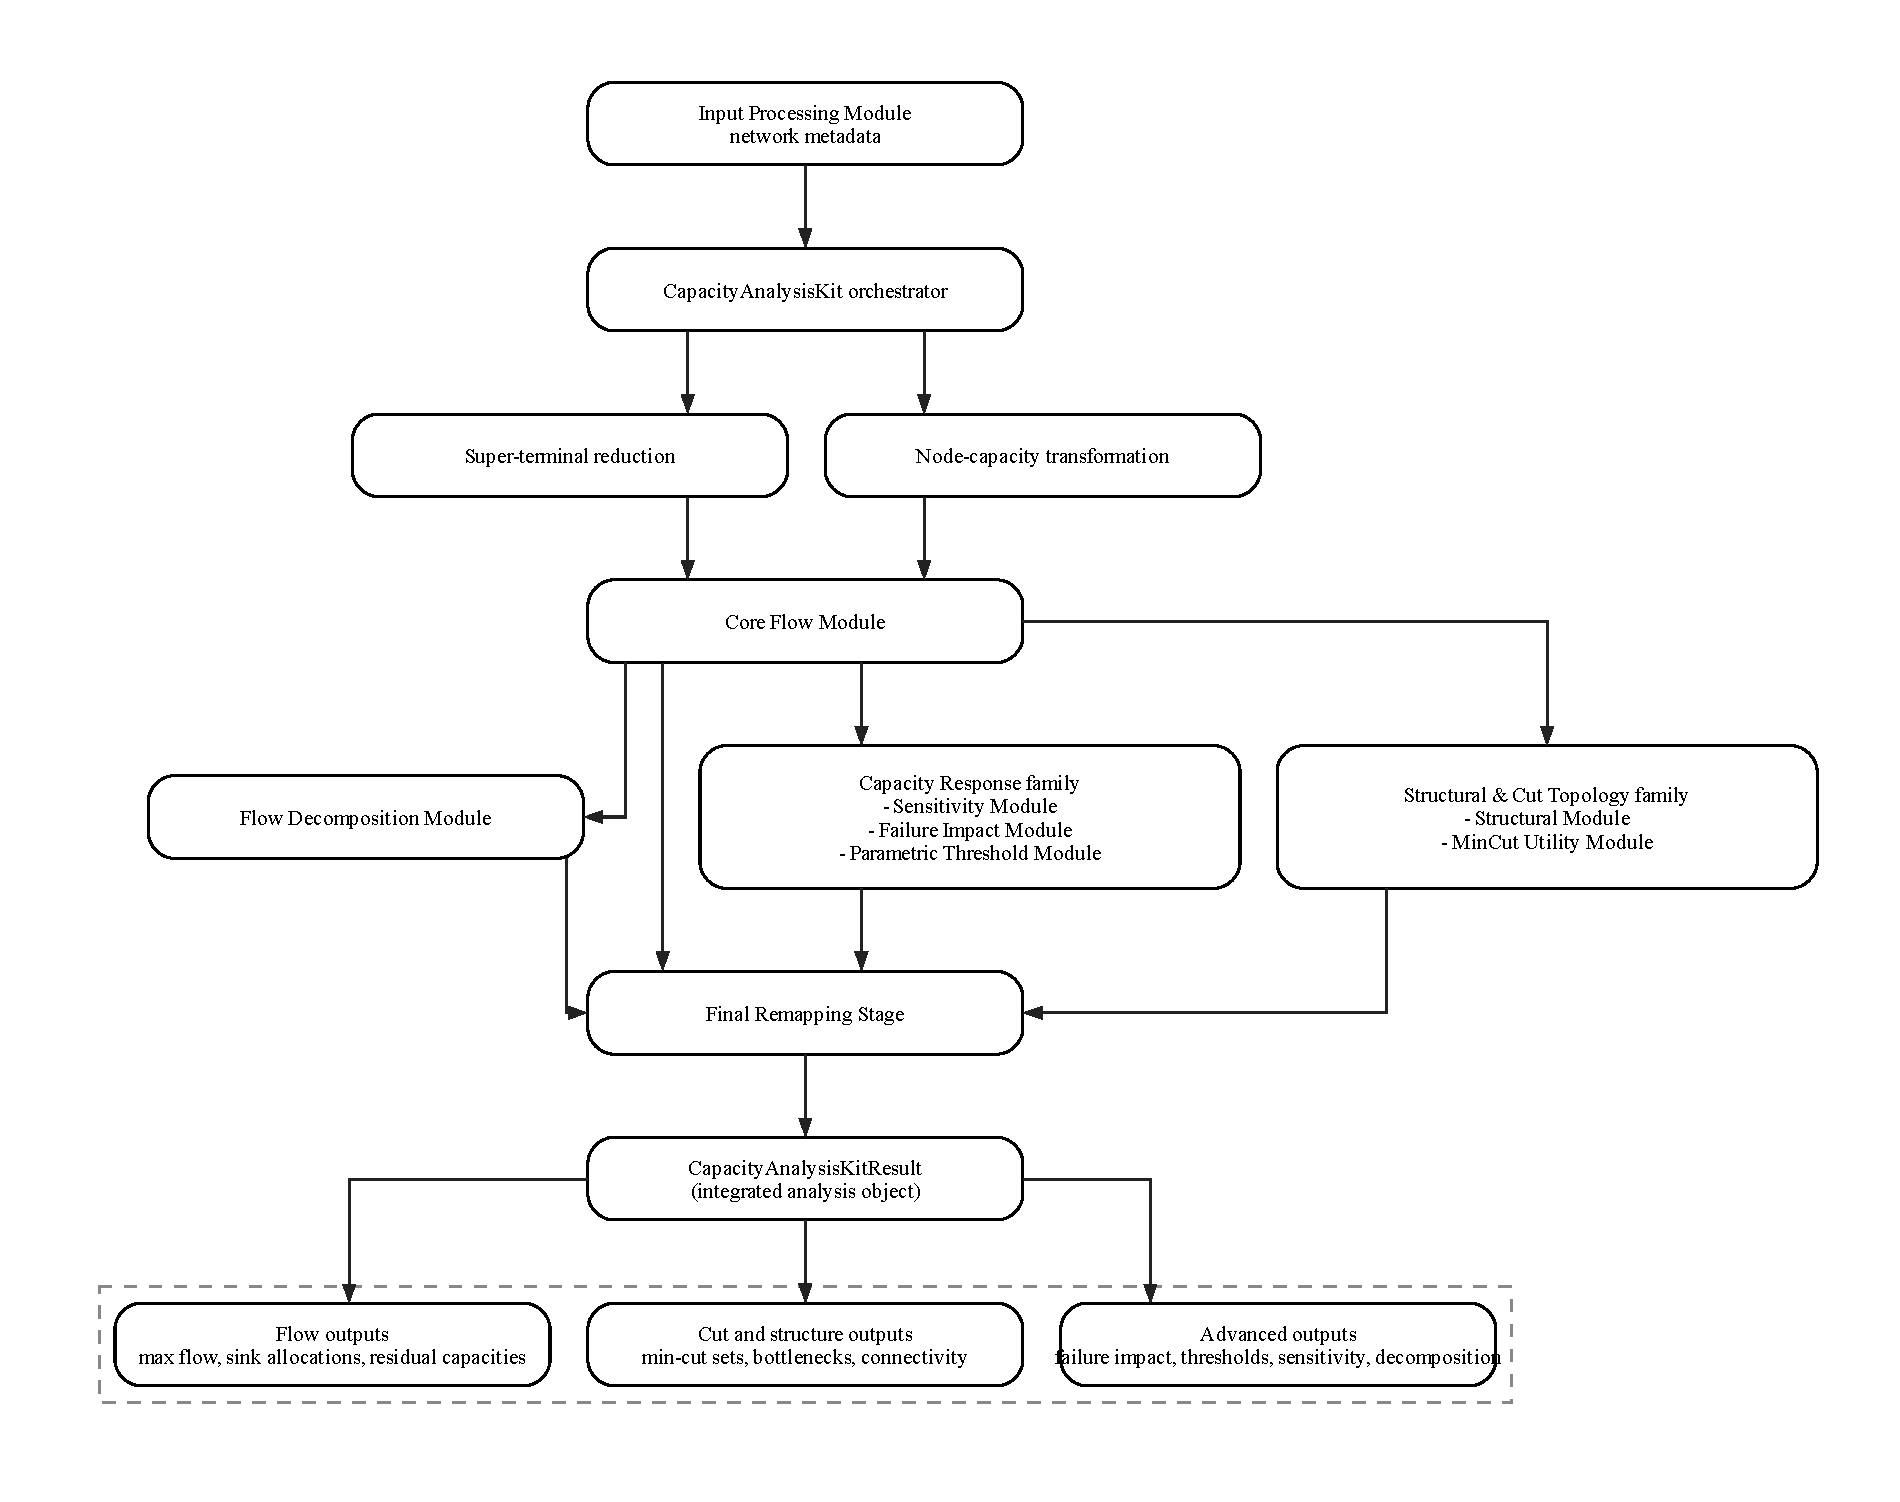
\includegraphics[height=0.6\textheight]{flow_toolkit_workflow.pdf}
\caption{Runtime workflow for the flow-capacity toolkit with available modules.}
\label{fig:flow_toolkit_workflow}
\end{figure}

\subsection{The binding cut and its lattice of equivalent cuts}
\label{sec:flow-mincut}
The flow module solvers all compute the max flow $F^\star$ by constructing a representative valid min-cut $S^\star$ in the given network $G$. This output by itself neither indicates nor guarantees that $S^\star$ is the only possible min-cut set in $G$.

The distinction matters for engineering decisions. Infrastructure systems are designed with redundancy, and in such networks several structurally distinct partitions of $V$ commonly have the same cut capacity $F^\star$.

While the baseline max flow value directly addresses the first analysis objective, the utility module uses the already-computed min-cut and residual graph to build the extended partition $S^{\star\star}$ and compute the full space of valid min-cuts. 

Let $R_T \subseteq V$ be the set of nodes reachable via backward traversal from 
$t^\star$ in $G_f$.

\begin{definition}[Extended Source Partition]
The extended source-side region is
\[
S^{\star\star} = V \setminus R_T,
\]
restricted to original graph nodes. Any node outside $R_T$ cannot reach the sink 
under the current flow state, so absorbing it into the source partition never 
increases cut capacity. Consequently $S^\star \subseteq S^{\star\star}$.
\end{definition}

\begin{definition}[Free Zone]
Given the extended partition, the free zone is
\[
\mathcal{F} = S^{\star\star} \setminus S^\star.
\]
Nodes in $\mathcal{F}$ can be assigned to either side of a minimum cut without 
affecting its capacity. Every minimum cut of $G$ under $f^\star$ takes the form 
$S = S^\star \cup R$ for some $R \subseteq \mathcal{F}$.
\end{definition}

The free zone size $|\mathcal{F}|$ itself determines the degeneracy of the bottleneck structure. When $|\mathcal{F}| = 0$ the minimum cut computed from the flow solver is unique and $S^\star$ is the only valid partition. For $|\mathcal{F}| > 0$ there are exactly 
$2^{|\mathcal{F}|}$ equivalent minimum cuts, meaning the cut boundary is not pinned 
to a single partition. 

Both the extended partition $S^{\star\star}$ and free zone $\mathcal{F}$ allow for a more complete picture of the bottleneck edge structure beyond what the representative cut alone provides. It then follows that two distinct edge sets can be derived directly from the lattice.

 The set of edges appearing in at least one minimum cut is \[ E_{\text{some}} = \{(u,v)\in E : f^\star_{uv} = c_{uv},\; u \in S^{\star\star},\; v \notin S^\star\}, \] and the set appearing in every minimum cut is \[ E_{\text{every}} = \{(u,v)\in E : f^\star_{uv} = c_{uv},\; u \in S^\star,\; v \in T^{\star\star}\}, \] where $T^{\star\star} = V \setminus S^{\star\star}$, and $E_{\text{every}} \subseteq E_{\text{some}}$ holds by construction. 

\subsubsection{Min-Cut Enumerator}
Given the residual lattice, the enumerator function in this utility module iterates over subsets $R \subseteq \mathcal{F}$ in binary counting order. Since each subset maps to a distinct minimum cut $S^\star \cup R$, every enumerated cut is guaranteed to be valid by lattice membership. The function exposes a \texttt{cut\_limit} parameter such that: if $2^{|\mathcal{F}|} \leq \texttt{cut\_limit}$ all minimum cuts are returned and \texttt{is\_complete} $=$ \texttt{true}; otherwise, the first \texttt{cut\_limit} cuts are returned with \texttt{is\_complete} $=$ \texttt{false}. This can be necessary in highly symmetric networks, where $|\mathcal{F}|$ can be large, making full enumeration intractable.



\subsection{Redundancy and single points of failure}
\label{sec:flow-structure}
The structural module identifies components whose importance follows from their position in $G$ alone, whatever the capacities. 

Understanding the route-level structure of $G$ is a prerequisite for any path-level fragility or flow-distribution analysis. The module exposes a base path enumerator function that performs a depth-first search on the topologically sorted iteration set of the graph object of Chapter~\ref{ch:system-model}. Since $G$ is a DAG, exact enumeration is always finite; however, highly redundant networks can admit exponentially many routes, so a \texttt{path\_limit} parameter bounds the number of enumerated paths and returns a sample and not the complete set $\mathcal{P}$.


\paragraph{Flow Decomposition.}
Two networks can share identical topology and the same $F^\star$ while concentrating flow through entirely different routes. During design decisions where multiple configurations are evaluated and per-route visibility is needed, this decomposition exposes how $f^\star$ is distributed across $\mathcal{P}$.

Given an optimal flow $f^\star$ and a set of flow-agnostic paths $\mathcal{P}$, for each path $P = (v_0, v_1, \ldots, v_k) \in 
\mathcal{P}$, the bottleneck flow contribution is the minimum flow on any edge along $P$:
\[
\phi(P) = \min_{i}\, f^\star_{v_i v_{i+1}},
\]
 Thus, the edge meeting this minimum must be the path's local bottleneck. Paths are sorted in descending order of $\phi(P)$ as a ranked decomposition of $f^\star$ into per-route contributions. Where the min-cut module's ranking informs global capacity upgrade decisions, this ranking informs targeted interventions at the route level. In a network supplying two distinct demand nodes via separate routes, the min-cut module points to the tightest cut edge across the whole network, whereas the decomposition identifies independently which component is constraining delivery to each demand node.

\paragraph{Structural Single Point of Failure Nodes.} 

\begin{definition}[Structural Single Point of Failure] 
A node $v \in V \setminus (S \cup T)$ is a SPOF node if $F^\star(G \setminus \{v\}) = 0$, where removing $v$ also removes all incident edges. A SPOF node is one through which every source-to-sink path must pass; its removal alone disconnects the network regardless of any capacity assignment. 
\end{definition} 

The candidate set is restricted to nodes lying on at least one $s$-$t$ path,
\[
\mathcal{C} = \bigl(\operatorname{fwd}(S) \cap 
\operatorname{bwd}(T)\bigr) \setminus (S \cup T),
\]
where $\operatorname{fwd}(S)$ and $\operatorname{bwd}(T)$ are the sets of nodes forward-reachable from $S$ and backward-reachable from $T$ in $G$ respectively. Nodes outside $\mathcal{C}$ lie on no $s$-$t$ path and cannot be SPOF nodes. For each $v \in \mathcal{C}$, a BFS is run on $G[V \setminus \{v\}]$; if no sink in $T$ is reachable from any source in $S$, $v$ is recorded as a SPOF node. The function requires one BFS per candidate and runs in $O(|\mathcal{C}| \cdot (|V| + |E|))$ time. 

In a node-capacitated network, a node appearing in the min-cut is not necessarily a SPOF node in this structural sense. A capacity-constrained node enters the cut-space by way of its split edges $(v_{\text{in}}, v_{\text{out}})$ with capacity $b_v$ and is not necessarily a structural choke-point in $G$. In these networks, a node 
can simultaneously be a flow-limiting bottleneck and a SPOF node.







\subsection{Throughput-limiting edges and their marginal values}
\label{sec:flow-sensitivity}
At optimality, the flow $f^\star$ partitions the edge set into two 
classes: edges carrying strictly less than their capacity, $f^\star_{uv} < c_{uv}$, and edges that carry exactly their capacity,
\[
f^\star_{uv} = c_{uv}.
\]
The latter are referred to as \emph{saturated edges} in this work. By the max-flow min-cut theorem, every minimum cut set is made up only of saturated edges; therefore, any augmenting path from $S$ to $T$ must cross at least one saturated edge. Since the binding constraint lies elsewhere, \emph{unsaturated edges} carry slack and are transparent to perturbation; increasing or decreasing their capacity by a small enough amount has little to no effect on $F^\star$. The Flow Sensitivity module focuses only on saturated edges, since they collectively form the capacity-critical boundary of the network. This module exposes the following three functions.

\paragraph{Critical Edge Ranking.}
A direct measure of an edge's failure impact is how much the max flow drops when that edge is disconnected from the network, referred to as edge criticality in this module. The function re-runs the flow solver on a modified network for each candidate. For each saturated edge $(u,v)$, the critical impact is:
\[
\Delta^\star_{uv} = F^\star(G,\, c) - 
F^\star\!\left(G,\, c^{(uv)}_0\right),
\]
where $c^{(uv)}_0$ denotes the capacity function with $c_{uv}$ set to zero and all other capacities unchanged. The function returns the edges in descending order of $\Delta^\star_{uv}$. 


\paragraph{Marginal Capacity Values.}
 Similar to the critical edge ranker, the function is scoped to saturated edges. For each saturated edge $(u,v)$, it quantifies the incremental gain in $F^\star$ per unit of additional capacity,
\[
\mu_{uv} = \frac{F^\star(G,\, c^{(uv)}_\delta) - 
F^\star(G,\, c)}{\delta},
\]
where $c^{(uv)}_\delta$ increases $c_{uv}$ by $\delta$ with all other capacities unchanged. 

In highly redundant networks, bypass routes often exist that can absorb rerouted flow and upgrade priorities are not always clear. In these systems, an edge can rank high for failure impact but have a lower marginal value. The critical edge function identifies which edges are most damaging to lose while the marginal capacity function complements this by identifying which ones are most worth upgrading.

\paragraph{Marginal Range.}
Both $\Delta^\star$ and $\mu$ are snapshot evaluations relative to the current capacity assignment $c$. Depending on the network structure, an edge with a low $\mu$ under the current inputs may become highly influential under different capacity values. This Marginal Range function evaluates the total range of influence a single edge $(u,v)$ can exert on $F^\star$:
\[
\mathcal{B}_{uv} = F^\star\!\left(G,\, c^{(uv)}_\infty\right) 
- F^\star\!\left(G,\, c^{(uv)}_0\right),
\]
where $c^{(uv)}_\infty$ sets $c_{uv} = \infty$ and $c^{(uv)}_0$ sets $c_{uv} = 0$, and all other capacities fixed. This function is analogous to the classical Birnbaum importance measure
$I_B(i) = \partial h(\mathbf{p})/\partial p_i$ (see~\cite{birnbaum1969}). However, the analogy is conceptual: $\mathcal{B}_{uv}$ is a deterministic throughput range, while the Birnbaum measure is a probability-weighted sensitivity.


\subsection{Failure impact and capacity degradation}
\label{sec:flow-failure}
The failure impact module models outright component failures and degraded operating states. 

\paragraph{Single and Combined Edge Failures.}
For a single failed edge $(u,v)$, the throughput impact is:
\[
\Delta_{uv} = F^\star(G,\, c) - F^\star\!\left(G,\, 
c^{(uv)}_0\right),
\]
where $c^{(uv)}_0$ sets $c_{uv} = 0$ with all other capacities unchanged and candidate edges are restricted to $E_{\text{some}}$.

Real failure events are not always isolated to a single component. A storm or substation fault in a power network can take down multiple edges simultaneously. Since the interaction between affected edges may open or close re-routing options, the combined impact of $k$ simultaneous failures is not in general the sum of their individual $\Delta_{uv}$ impacts.

The $k$-edge failure function generalises the single failure case to any set of $k$ edges removed simultaneously. For a combination $\mathcal{K} \subseteq E_{\text{some}}$ with $|\mathcal{K}| = k$, the combined impact is:
\[
\Delta_{\mathcal{K}} = F^\star(G,\, c) - 
F^\star\!\left(G,\, c^{(\mathcal{K})}_0\right),
\]
where $c^{(\mathcal{K})}_0$ sets $c_{uv} = 0$ for all $(u,v) \in \mathcal{K}$. 
All $\binom{|E_{\text{some}}|}{k}$ combinations require one re-solve each. In practice, because $\binom{|E_{\text{some}}|}{k}$ grows rapidly with $k$, this function is most tractable for $k = 2$ or $k = 3$ depending on the size and density of the network. The function returns a complete ranking of $k$-edge failure scenarios by throughput impact.

\paragraph{Capacity Degradation Scenarios.}
Infrastructure components do not always fail completely. Partial blockage or degraded components are more likely to present as a 
reduction in $c_{uv}$ without complete loss. Additionally, a domain expert working across multiple network states may want to compare the effect of varying input capacities and operating conditions. This function is intended to be used to efficiently compute the full $F^\star$ picture across all scenarios without needing to re-run the input processing or baseline solve steps for each.
The degradation function accepts either an explicit override dictionary specifying new capacities for individual edges, or a uniform scale factor 
$\alpha \in [0,1]$ applied to all finite capacities,
\[
c'_{uv} = \alpha \cdot c_{uv}, \qquad \forall (u,v) \in E.
\]





\subsection{Degradation and upgrade thresholds}
\label{sec:flow-parametric}

The previous modules treat edge capacities as fixed and analyse the network's response to perturbations around them. The threshold module inverts this perspective. Given a required demand level $D_t \leq F^\star$ to be met, it determines what capacity each edge must have for the network to meet that target delivery level. It is therefore a planning tool.

This module uses a structural property of $F^\star$: it is piecewise linear in any single edge capacity $c_e$ with all others fixed. Each linear segment maps to a fixed min-cut partition $S^\star$, over which the threshold satisfying $F^\star(c_e) = D_t$ can be recovered analytically. Therefore, breakpoints must occur exactly where the min-cut partition shifts, i.e.\ where a change in $c_e$ causes a different set of edges to become the binding bottleneck.

\paragraph{Degradation Threshold.}
For a target edge $(u,v)$ and a required flow level $D_t$, the degradation threshold $c^\dagger_{uv}$ is the minimum capacity the edge must retain for $F^\star$ to remain at least $D_t$:
\[
c^\dagger_{uv} = \inf\bigl\{c \in [0, c_{uv}] : 
F^\star(G,\, c^{(uv)}_c) \geq D_t \bigr\},
\]
where $c^{(uv)}_c$ denotes the capacity function with $c_{uv}$ replaced by $c$. The degradation margin $c_{uv} - c^\dagger_{uv}$ is the slack available before the service level is breached. The module ranks edges by ascending degradation margin, so the most vulnerable edges appear first. A small margin can be interpreted as the edge is close to becoming a binding constraint on $D_t$, while a large margin means the edge can absorb substantial capacity loss without service impact.

The threshold is located by a partition-change recursion. Starting from the known endpoints $c_e = 0$ and $c_e = c_{uv}$, the algorithm evaluates $F^\star$ at the midpoint and compares the resulting min-cut partition to those at the endpoints. If both endpoints share the same partition, the segment is linear and the threshold is solved analytically. If the partitions differ, the interval contains a breakpoint and the recursion descends into the sub-interval containing $D_t$. This continues until the threshold is isolated to a partition-constant segment, where it is computed exactly. The result is exactly the capacity value at which $F^\star$ crosses $D_t$.

Two degenerate cases are handled explicitly. If $F^\star(c_e = 0) \geq D_t$, the edge can degrade to zero without breaching the target. If $F^\star(c_e = c_{uv}) < D_t$, the target is unachievable even at the current capacity, meaning the bottleneck lies entirely elsewhere and this edge cannot help.

\paragraph{Upgrade Threshold.}
If $F^\star < D_t$ under the current capacity assignment, the upgrade threshold is the minimum capacity $(u,v)$ must have for $F^\star$ to first reach $D_t$. Since the required capacity may exceed $c_{uv}$, the upper search bound is not known in advance. The algorithm uses a doubling search to bracket the threshold interval, repeatedly doubling the trial capacity until $F^\star \geq D_t$, then applies the same partition-change recursion to locate it exactly.

An edge case arises when the edge is not on any minimum cut: expanding its capacity cannot raise $F^\star$ regardless of how large $c_{uv}$ becomes. The doubling search detects this when $F^\star$ stops increasing before reaching $D_t$ and returns \texttt{upgrade\_ineffective} $=$ \texttt{true}, indicating that reaching $D_t$ requires addressing a different bottleneck. 

When no explicit target is supplied, the module defaults to $D_t = 0.9 \cdot F^\star$.




\section{Cost}
\label{sec:flow-cost}
The total computational cost of any derived analysis is the product of the per-solve cost of the chosen max-flow algorithm and the number of solver calls required. Repeated-solve tasks scale with solve count, which is the dominant cost driver in practice. Per-solve costs are summarised in Table~\ref{tab:solver_comparison}, and Table~\ref{tab:flowcap_complexity} gives the per-task cost of every module function in units of one solve.

\begin{longtable}{l l l r}
\toprule
\textbf{Module} & \textbf{Function} & \textbf{Operation} & \textbf{Complexity} \\
\midrule
\endfirsthead
\toprule
\textbf{Module} & \textbf{Function} & \textbf{Operation} & \textbf{Complexity} \\
\midrule
\endhead
\bottomrule
\footnotetext[1]{Bounded by \texttt{cut\_limit}; $|\mathcal{F}|$ is free-zone size.}
\footnotetext[2]{Bounded by \texttt{path\_limit}; $\ell$ = max path length.}
\footnotetext[3]{Throws if $\binom{|E_s|}{k} > 10{,}000$.}
\endfoot
\multicolumn{4}{l}{\small\textit{Base Solver}} \\
Base & Edmonds-Karp & BFS augmenting path & $O(VE^2)$ \\
Base & Dinic & Level graph + blocking & $O(V^2E)$ \\
Base & Push-Relabel & Preflow relabeling & $O(V^3)$ \\[2pt]
Node-Cap & Split transformation & Graph transform & $O(V+E)$ \\
Node-Cap & Solve (split) & Solver on $2V, 2E$ & $O(T_{\text{solver}})$ \\
\multicolumn{4}{l}{\small\textit{Min-Cut Utility}} \\
Min-Cut & \texttt{cut\_edges} & Extract partition & $O(E)$ \\
Min-Cut & \texttt{edges\_some} & BFS + filter & $O(E + T_s)$ \\
Min-Cut & \texttt{edges\_every} & Reachability & $O(V+E)$ \\
Min-Cut & \texttt{enumerate} & Lattice ($2^{|\mathcal{F}|}$) & $O(2^{|\mathcal{F}|} \cdot E)$\footnotemark[1] \\[2pt]
\multicolumn{4}{l}{\small\textit{Structural}} \\
Struct & \texttt{spof\_nodes} & BFS per candidate & $O(|\mathcal{C}|(V+E))$ \\
Struct & \texttt{enumerate\_paths} & DFS on DAG & $O(|\mathcal{P}|)$\footnotemark[2] \\
Struct & \texttt{path\_flow} & Per-path scan & $O(|\mathcal{P}| \ell)$ \\
Struct & \texttt{redundancy} & Menger (unit cap) & $O(|E_c| T_s)$ \\[2pt]
\multicolumn{4}{l}{\small\textit{Flow Sensitivity}} \\
Sens & \texttt{critical\_edges} & Zero-cap solves & $O(|E_{\text{sat}}| T_s)$ \\
Sens & \texttt{marginal\_capacity} & $+\delta$ solves & $O(|E_{\text{sat}}| T_s)$ \\
Sens & \texttt{marginal\_range} & Range evals & $O(|E_{\text{some}}| T_s)$ \\[2pt]
\multicolumn{4}{l}{\small\textit{Failure Impact}} \\
Fail & \texttt{single\_edge} & Per-edge solves & $O(|E_{\text{some}}| T_s)$ \\
Fail & \texttt{k\_edge} & Per-combination & $O(\binom{|E_s|}{k} T_s)$\footnotemark[3] \\
Fail & \texttt{degradation} & Per-scenario & $O(|S| T_s)$ \\[2pt]
\multicolumn{4}{l}{\small\textit{Parametric Threshold}} \\
Param & \texttt{degrade} & Partition recursion & $O(\lg(c/\varepsilon) T_s)$ \\
Param & \texttt{upgrade} & Doubling + recurse & $O(\lg^2(c/\varepsilon) T_s)$ \\
Param & \texttt{all\_degrade} & Per edge & $O(|E_c| \lg(c/\varepsilon) T_s)$ \\[2pt]
\caption{Per-task computational complexity for the flow capacity toolkit. $T_s$ denotes the cost of a single max-flow solve under the chosen algorithm.}
\label{tab:flowcap_complexity}
\end{longtable}




\section{Validation}
\label{sec:flow-validation}

Every output of the toolkit was checked against a computation that does not use its solvers.
The checks were run on a set of twelve networks, the ten DAGs of the Chapter~\ref{ch:critical-path}
validation set with the three published drone designs in place of the larger drone network,
plus the PSPLIB instance of Chapter~\ref{ch:critical-path}, each with integer capacities drawn
uniformly from $[1, 20]$ per edge from a recorded seed, and four of them with node capacities
drawn in the same way. The networks, seeds and files are listed in
Appendix~\ref{app:full-results}.

The maximum-flow value was computed by all three solvers and by the \texttt{GraphsFlows.jl}
library \cite{graphsflows} as an external oracle. On every network the three solvers agree
with each other and with the oracle exactly, and every returned flow passes the three
post-solve checks: capacity feasibility on every edge, conservation at every transit node, and
equality of the flow value and the reported cut capacity.

The structural outputs were checked by brute force. Every enumerated minimum cut was checked
to have capacity equal to the maximum flow and to disconnect the sources from the sinks, and
on networks with at most twenty candidate edges every edge subset that disconnects was
enumerated and the reported cuts were confirmed to be exactly the minimal ones of minimum
capacity. The two derived edge sets of Section~\ref{sec:flow-mincut} were checked against
the same enumeration: the edges reported in every minimum cut must equal the intersection of
the enumerated cuts and the edges reported in some minimum cut their union. This check was
added after the interface of Chapter~\ref{ch:front-end} showed, on a 23-node network, a set
of edges in every cut that lay entirely on the source side of the unique cut; the function
had taken the complement of the sink-reachable set, and the earlier checks had tested the
enumerated cuts without testing the two sets derived from them. Every reported saturated edge was checked to carry flow equal to its capacity.
Single points of failure and the single-edge failure ranking were checked by removing each
node and each edge in turn and recomputing the maximum flow with the oracle, exhaustively on
the small networks and on a sample of between fifteen and forty removals on the large ones.
Each degradation threshold was checked by evaluating the oracle just below and just above it,
and by locating the threshold independently by bisection. The edge-disjoint path count was
checked against a unit-capacity oracle flow, which is Menger's theorem. The node-capacitated
flow was checked against the oracle applied to the split graph, and the several-source and
several-sink construction is exercised by every network in the set. All checks passed on all
twelve networks.

The last of these checks found an error. On the IEEE network of Section~\ref{sec:flow-rts24},
where ten of twenty-four buses carry a node capacity and the rest do not, the node-splitting
transformation assigned the entry and exit nodes identifiers $2v$ and $2v+1$, which collide
with the identifiers of unsplit nodes when only some nodes are split and the identifiers are
small and consecutive. None of the twelve corpus networks had exposed it, because in each of
them every node or no node carried a capacity. The transformation now assigns identifiers
above the largest identifier in the network, and the corrected code gives identical results on
every network that had passed before. The change is described in Chapter~\ref{ch:julia-package}.

\section{Case Studies}
\label{sec:flow-cases}

Timings in this section are wall-clock measurements on a single core of the second call in a
warm process, so that just-in-time compilation is excluded. The convention is stated in
Appendix~\ref{app:full-results}.

\subsection{A worked example on a synthetic network}
\label{sec:flow-worked}
The modules are first shown together on a synthetic network built so that each of them has something to report. It is a worked example; the case study follows in Section~\ref{sec:flow-rts24}. The network is a multi-source, multi-sink capacitated DAG with 43 nodes, 107 directed edges. The network represents a distribution system that moves a resource between dispersed locations. As shown in Figure~\ref{fig:flow_bm_networks}, it is structured as an 8-layer hierarchy:

\begin{itemize}
    \item \textbf{Origin nodes} (blue): five source nodes, over-provisioned so the supply zone does not form the binding bottleneck.
    \item \textbf{Hub nodes} (green): eight intermediate relay nodes with high fan-out capacities.
    \item \textbf{Processing nodes} (red, node-capacitated) and \textbf{bypass nodes} (orange, node-capacitated): the processing corridor carries the bulk of flow; the bypass is a lightweight alternative with tighter node constraints.
    \item \textbf{Trunk and secondary nodes} (purple, brown): distribute flow through a re-converging structure toward the gateway layer.
    \item \textbf{Dispatch gateways} (light blue, node-capacitated): two gateways assigned equal edge capacity of 17 by design.
    \item \textbf{Distribution combiner} (pink): aggregates all gateway flow before fan-out to the sinks.
    \item \textbf{Sink nodes} (grey): seven demand nodes, each with incoming edge capacity 6.
\end{itemize}
Based on this layered structure, edge and node capacity assignments are chosen so that binding bottlenecks emerge at specific layers under the different analysis methods. Edge capacities in Layers~1--5 are scaled by a factor of 2 relative to the gateway layer. In this way, the gateway layer governs $F^\star$ under the edge-only solution. Similarly, to compute a measurable reduction in $F^\star$, the processing node capacities are set to bind to the node-capacitated solve.

Two configurations of the same system are compared to show the effect of feeder reinforcement (Figures~\ref{fig:network_a} and~\ref{fig:network_b}). 
Both configurations keep the same topology and differ in their feeder capacities. The comparison tests whether the bottleneck structure changes when the throughput does not. 

Configuration A is a symmetric design with balanced feeder-edge capacities and a limited direct bypass to sink 4. The capacity is set below the sink's 6-unit limit so that the bypass delivers partial service. Configuration B's asymmetric gateway structure produces non-trivial parametric upgrade thresholds and non-zero marginal-range values. This version has larger feeder capacities from secondary nodes into both gateways.
 
Table~\ref{tab:config_comparison} summarises the key structural differences between the two. The expectation is that two designs may yield the same max-flow value while differing in saturation pattern and in the set of minimum cuts, because their feeder capacities differ.



\subsubsection{Two configurations compared}

The base flow solver run returns $F^\star = 37.0$, with $\texttt{mincut\_capacity} = 37.0$ for both networks, which is the maximum feasible flow for the system as built. However, $F^\star$ alone does not distinguish the two designs. As shown in Table~\ref{tab:config_comparison}, the two networks still differ in structure: Configuration A carries more saturated edges, has a non-empty free zone and admits several equivalent minimum cuts, while the minimum cut in Configuration B is unique. The two designs have the same throughput under different constraints, which is what the remaining modules distinguish.

\begin{table}[htbp]
\centering
\caption{Configuration comparison summary.}
\label{tab:config_comparison}
\begin{tabular}{lcc}
\toprule
Metric & Configuration A & Configuration B \\
\midrule
$F^*$                                        & 37.0           & 37.0           \\
\texttt{saturated\_edges}                    & 41             & 35             \\
\texttt{free\_zone\_size}                    & 2              & 0              \\
\texttt{min\_cuts}                           & 4              & 1              \\
\texttt{SPOF\_nodes}                         & 0              & 0              \\
\texttt{upgrade\_ineffective} (gateway edges) & \texttt{true} & \texttt{false} \\
\bottomrule
\end{tabular}
\end{table}

The difference is one of structural flexibility against bottleneck localisation. In Configuration A the free-zone nodes are $\{134,135\}$. The cut lattice is therefore wider, and $E_{\text{every}}$ and $E_{\text{some}}$ differ. The gateway edges $134 \to 136$ and $135 \to 136$ appear in $E_{\text{some}}$ but not in $E_{\text{every}}$, so neither is a universal failure mode on its own. Cut 4 has only 3 crossing edges while Cut 1 has 13, both at capacity 37 (Table~\ref{tab:mincut_enumeration_config_a}). In Configuration B, feeder-capacity reinforcement pins the cut to a unique partition: free-zone size collapses to 0 and the gateway edges move into $E_{\text{every}}$. The choice between configurations depends on the optimisation target: Configuration A offers more structural redundancy and cut diversity, while Configuration B offers tighter bottleneck localisation and actionable upgrade thresholds.

\paragraph{Bypass edge and single points of failure.}

The direct bypass edge $132 \to 140$ improves $\texttt{sink\_4}$ service with capacity 3, below the sink-side limit of 6. The same edge raises redundancy scores for all secondary-to-gateway connections from 2 to 3, so redundancy improves across the whole gateway-feeding layer, well beyond the nodes it directly connects.

Without this edge, node 136 is the only SPOF node: every source-to-sink path passes through it and $F^\star(G \setminus \{136\}) = 0$. Adding $132 \to 140$ gives $F^\star(G \setminus \{136\}) = 3 > 0$, removing node 136 from the SPOF set, and both configurations report $\texttt{spof\_nodes} = \emptyset$. However, only $\texttt{sink\_4}$ has an alternative path, so all other flow still passes through the combiner. Running the capacity degradation module with node 136 removed confirms this: $F^\star$ drops to 3, exposing the network's continued vulnerability to combiner failure despite the absence of a formal SPOF classification.

\paragraph{Node-capacitated analysis.}
When node capacities are enabled, both configurations still return the same result: a 7-unit loss down to $\texttt{node\_cap\_max\_flow}=30.0$. The same six Layer~3 nodes $\{114,115,116,117,118,119\}$ saturate in both cases. This tells the designer where to act: once these node limits are active, changing gateway-edge capacities does not change the outcome.

The flow loss is not shared evenly across demand nodes (Figure~\ref{fig:sink_flow_heatmap}). \texttt{sink\_1} (137) falls from 4.0 to 0.0, so it loses service completely. \texttt{sink\_2} (138) falls from 6.0 to 3.0, while sinks 139--143 stay at their previous levels. Total flow alone does not show this.

To test a direct fix, a single-node upgrade sweep was run on nodes 114--119 (Table~\ref{tab:node_upgrade_sweep}). Upgrading any one of these nodes restores \texttt{sink\_1} to its edge-only service level and returns total flow to $F^\star=37.0$ in both configurations. The required increment is identical for all six nodes, while the three node pairs reach different absolute targets because they start from different capacities. The six upgrades therefore have the same effect on throughput, and the choice between them is settled by delivery constraints such as cost, installation effort and access.

\begin{table}[htbp]
\centering
\caption{Node-upgrade sweep (Configurations A and B give identical results): minimum single-node capacity increase required to restore \texttt{sink\_1} service under the node-capacitated solve.}
\label{tab:node_upgrade_sweep}
\begin{tabular}{lccc}
\toprule
Node & Current $b_v$ & Required $\Delta b_v$ & New $b_v$ \\
\midrule
114 (\texttt{processing\_A}) & 5.0 & 7.0 & 12.0 \\
115 (\texttt{processing\_B}) & 5.0 & 7.0 & 12.0 \\
116 (\texttt{processing\_C}) & 7.0 & 7.0 & 14.0 \\
117 (\texttt{processing\_D}) & 7.0 & 7.0 & 14.0 \\
118 (\texttt{bypass\_E})     & 3.0 & 7.0 & 10.0 \\
119 (\texttt{bypass\_F})     & 3.0 & 7.0 & 10.0 \\
\bottomrule
\end{tabular}
\end{table}

\paragraph{Flow decomposition results.}

Flow decomposition shows that both configurations achieve the same total throughput ($F^\star=37.0$) with very similar route-level allocation. Configuration A decomposes into 27 components and Configuration B into 25, so the difference is small and does not change the main delivery pattern. In both cases, the largest single component carries 3.0 units on a path bottlenecked at $(114\to120)$, and most remaining components are paths carrying 2.0 or 1.0 units distributed across the processing and bypass corridors.

This agrees with the structural results above. The A/B edge-capacity changes alter which secondary-to-gateway edges appear as local path bottlenecks, but they do not create a different high-level flow-allocation picture. The dominant route family still passes through the same Layer 3 processing/bypass region and then through the combiner to sinks, with the direct bypass to sink 4 contributing only partial service. At decomposition level, the two designs differ in local edge pressure more than in overall route usage.

\paragraph{Sensitivity analysis.}

Sensitivity ranking shows a tiered pattern in Configuration A (Table~\ref{tab:critical_edges_config_a}). Single-edge impact falls into four tiers, from the two gateway-to-combiner edges $(134\to136)$ and $(135\to136)$ at the head of the ranking down to the outer feeders at the foot. Removing either gateway edge reduces throughput by about 46 per cent. Below the gateway pair sits a tier of secondary-to-gateway feeders, and the tier below that contains the direct bypass edge $(132\to140)$, which therefore carries the same single-edge impact as several of those feeders. In total, 15 edges have non-zero single-edge impact in Configuration A.

\begin{table}[htbp]
\centering
\caption{Full ranked single-edge sensitivity results for Configuration A (all non-zero $\Delta F^\star$ edges).}
\label{tab:critical_edges_config_a}
\begin{tabular}{lccc}
\toprule
Rank & Label & $\Delta F^\star$ & \texttt{perturbed\_flow} \\
\midrule
1 & \texttt{dispatch\_gateway\_west->distribution\_combiner} & 17.0 & 20.0 \\
2 & \texttt{dispatch\_gateway\_east->distribution\_combiner} & 17.0 & 20.0 \\
3 & \texttt{secondary\_a->dispatch\_gateway\_west} & 4.0 & 33.0 \\
4 & \texttt{secondary\_c->dispatch\_gateway\_east} & 4.0 & 33.0 \\
5 & \texttt{secondary\_d->dispatch\_gateway\_west} & 4.0 & 33.0 \\
6 & \texttt{secondary\_f->dispatch\_gateway\_east} & 4.0 & 33.0 \\
7 & \texttt{secondary\_b->dispatch\_gateway\_west} & 3.0 & 34.0 \\
8 & \texttt{secondary\_b->dispatch\_gateway\_east} & 3.0 & 34.0 \\
9 & \texttt{secondary\_e->dispatch\_gateway\_west} & 3.0 & 34.0 \\
10 & \texttt{secondary\_e->dispatch\_gateway\_east} & 3.0 & 34.0 \\
11 & \texttt{secondary\_e->sink\_4} & 3.0 & 34.0 \\
12 & \texttt{secondary\_c->dispatch\_gateway\_west} & 2.0 & 35.0 \\
13 & \texttt{secondary\_d->dispatch\_gateway\_east} & 2.0 & 35.0 \\
14 & \texttt{secondary\_a->dispatch\_gateway\_east} & 1.0 & 36.0 \\
15 & \texttt{secondary\_f->dispatch\_gateway\_west} & 1.0 & 36.0 \\
\bottomrule
\end{tabular}
\end{table}

\begin{figure}[htbp]
\centering

\begin{subfigure}[t]{\textwidth}
    \centering
    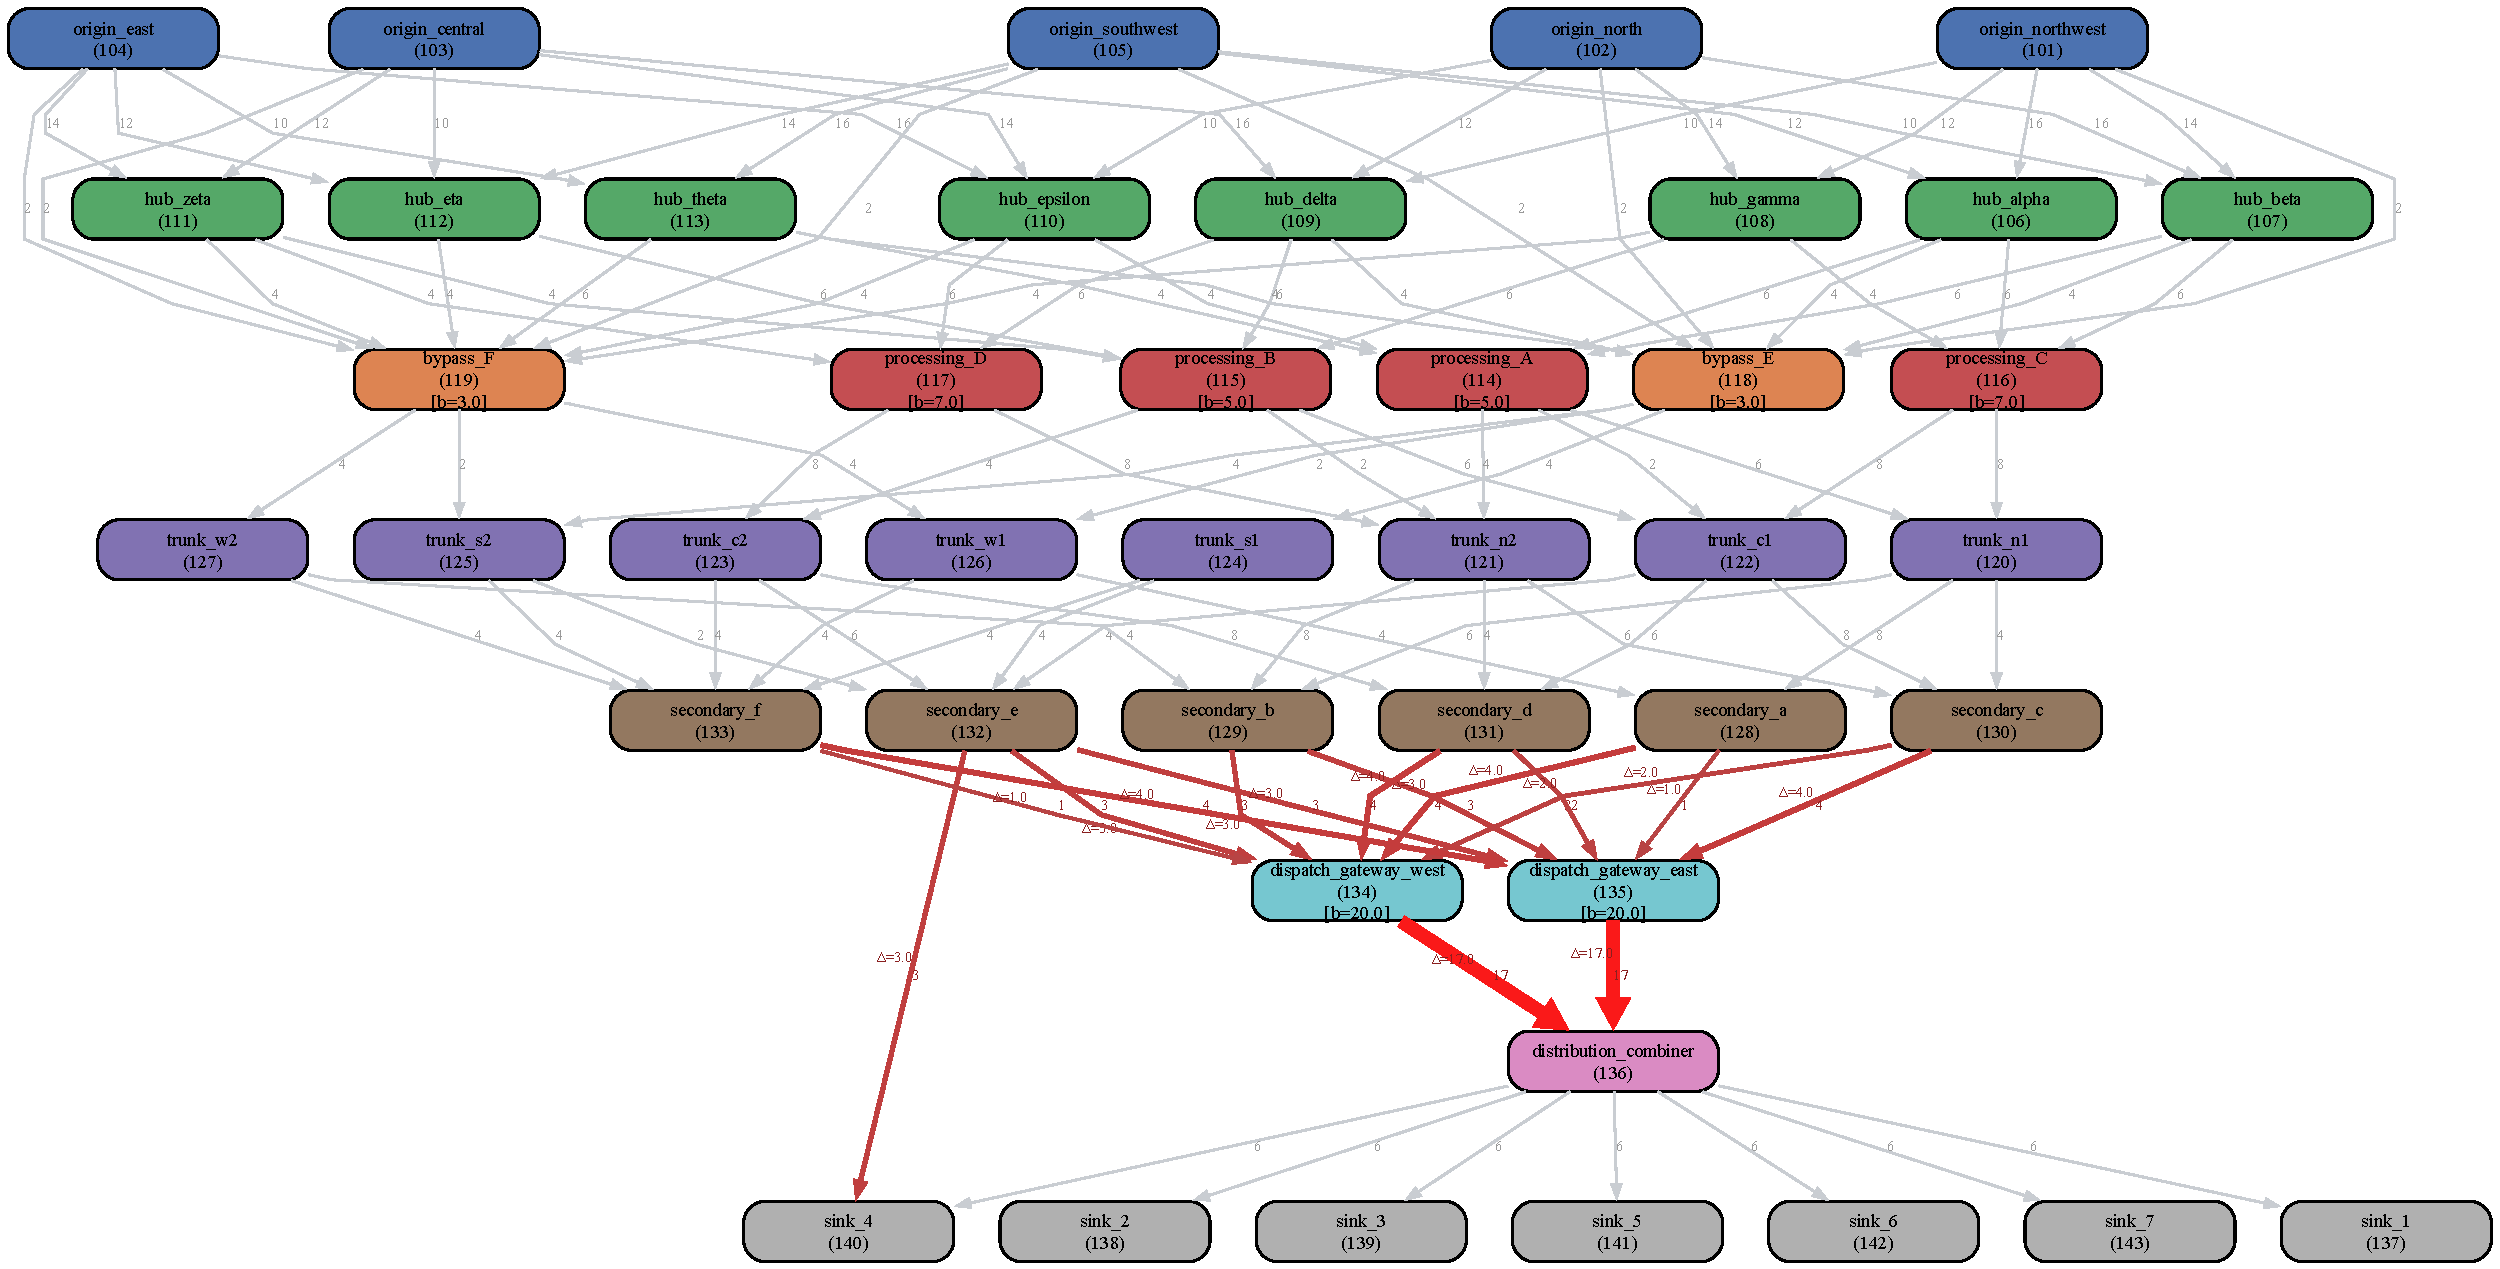
\includegraphics[width=\textwidth, keepaspectratio]{critical_overlay_config_a}
    \caption{Configuration A critical-edge overlay. Edge emphasis (colour/width) is proportional to non-zero $\Delta F^\star$.}
    \label{fig:critical_overlay_a}
\end{subfigure}

\vspace{0.8em}

\begin{subfigure}[t]{\textwidth}
    \centering
    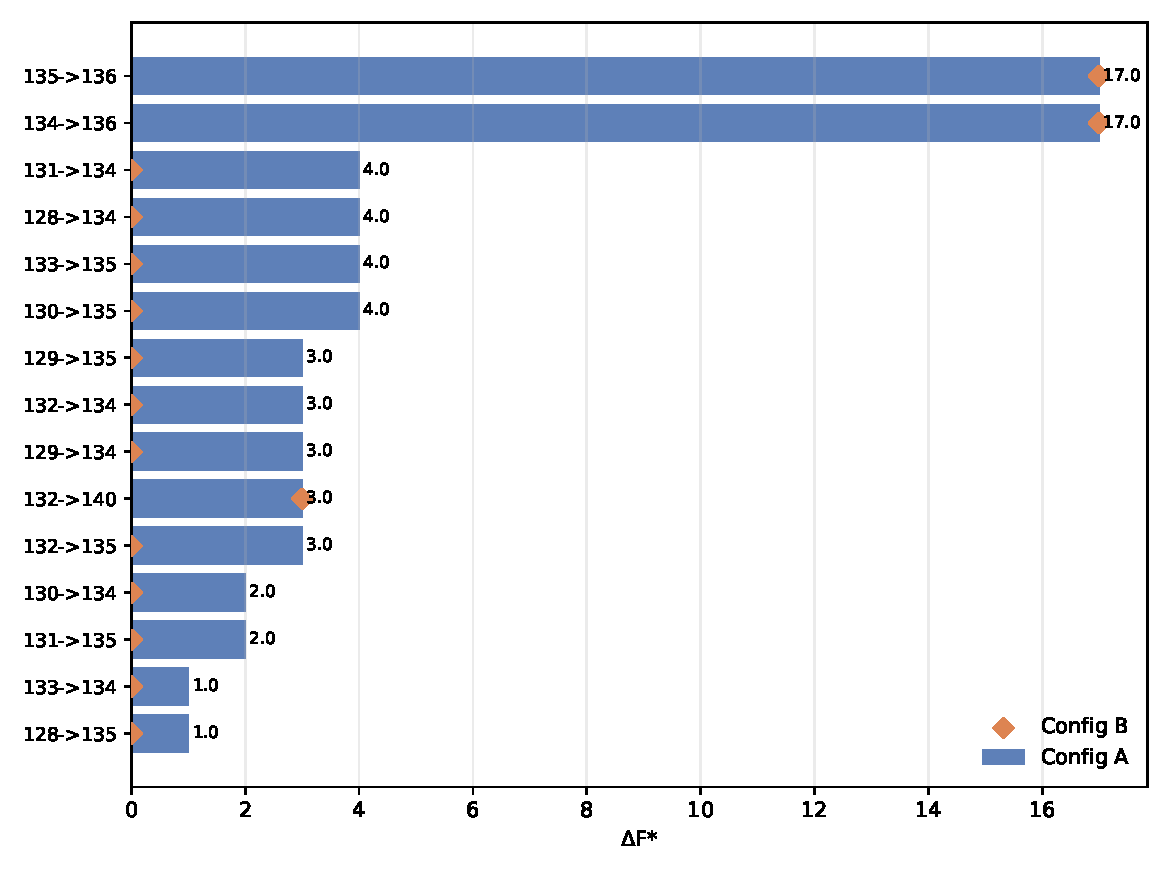
\includegraphics[width=\textwidth, keepaspectratio]{critical_bars_config_ab}
    \caption{Ranked non-zero single-edge sensitivity for Configurations A and B.}
    \label{fig:critical_bars_ab}
\end{subfigure}

\caption{Single-edge sensitivity in Configuration A and cross-configuration rank comparison (A vs B).}
\label{fig:sensitivity_two_panel}
\end{figure}

Configuration B is more concentrated: only three edges have non-zero impact, $(134\to136)$, $(135\to136)$, and $(132\to140)$, while all other evaluated edges give $\Delta^\star=0$ (Table~\ref{tab:critical_edges_config_b}). This means the feeder-capacity reinforcement in B absorbs any single feeder-edge loss through rerouting, so feeder removals no longer reduce $F^\star$ individually. The non-zero set therefore collapses from 15 edges in A to 3 in B.

\begin{table}[htbp]
\centering
\caption{Full ranked single-edge sensitivity results for Configuration B (all non-zero $\Delta F^\star$ edges).}
\label{tab:critical_edges_config_b}
\begin{tabular}{lccc}
\toprule
Rank & Label & $\Delta F^\star$ & \texttt{perturbed\_flow} \\
\midrule
1 & \texttt{dispatch\_gateway\_west->distribution\_combiner} & 17.0 & 20.0 \\
2 & \texttt{dispatch\_gateway\_east->distribution\_combiner} & 17.0 & 20.0 \\
3 & \texttt{secondary\_e->sink\_4} & 3.0 & 34.0 \\
\bottomrule
\end{tabular}
\end{table}

\paragraph{Failure impact.}
The two-edge failure ranking confirms that the dominant pair is simultaneous loss of $(134\to136)$ and $(135\to136)$, with drop 34.0 and perturbed flow 3.0. This is much larger than the next group (drop 21.0), and follows from the single-edge pattern shown in Figure~\ref{fig:sensitivity_two_panel}. In Configuration B, the same gateway-pair dominance remains, while the non-zero failure set is more concentrated because feeder reinforcement absorbs most single-edge feeder losses through rerouting.

\paragraph{Degradation trajectory.}
The degradation trajectories are identical for Configurations A and B at all tested scale factors. The solved values are: $\alpha=1.0 \rightarrow 37.0$, $\alpha=0.9 \rightarrow 33.3$, $\alpha=0.8 \rightarrow 29.6$, $\alpha=0.7 \rightarrow 25.9$, $\alpha=0.6 \rightarrow 22.2$, and $\alpha=0.5 \rightarrow 18.5$. These points follow the linear relation
\[
F^\star(\alpha)=37\alpha
\]
over the tested interval.

The A/B curves that coincide point-for-point (Figure~\ref{fig:degradation_trajectory}) indicate that the feeder-capacity differences that separate A and B under single-edge sensitivity do not produce a different global response under a uniformly scaled network-wide degradation.

\paragraph{Parametric thresholds.}
Parametric thresholds separate an edge's criticality from its upgradeability, and Table~\ref{tab:parametric_comparison} sets the two measures side by side for the three edges on which the configurations differ. In Configuration A, the gateway edges $(134\to136)$ and $(135\to136)$ need an infinite capacity increase to raise throughput at all, so they are upgrade-ineffective despite their high impact in the sensitivity ranking. In Configuration B, the same gateway edges become upgrade-effective at a finite capacity. Both configurations have zero margin on these edges: any capacity loss below the current level immediately reduces $F^\star$.

This difference is explained by upstream supply. In Configuration A, supply into each gateway is already capped at the current gateway-edge capacity, so increasing gateway-edge capacity alone cannot raise throughput. In Configuration B, feeder reinforcement creates upstream headroom, so gateway-edge upgrades can increase $F^\star$.

The bypass edge $(132\to140)$ is upgrade-effective in both configurations, unlike the gateway edges. The contrast between the two configurations in upgrade feasibility is therefore concentrated at the gateway edges.

\begin{table}[htbp]
\centering
\caption{Parametric threshold and marginal range comparison 
for key edges.}
\label{tab:parametric_comparison}
\begin{tabular}{lcccc}
\toprule
Edge & \multicolumn{2}{c}{Configuration A} & \multicolumn{2}{c}{Configuration B} \\
\cmidrule(lr){2-3}\cmidrule(lr){4-5}
 & Upgrade & $\mathcal{B}_{uv}$ & Upgrade & $\mathcal{B}_{uv}$ \\
\midrule
$134\to136$ & ineffective & 17.0 & $+1.0$ & 23.0 \\
$135\to136$ & ineffective & 17.0 & $+1.0$ & 23.0 \\
$132\to140$ & $+1.0$      & 10.0 & $+1.0$ & 16.0 \\
\bottomrule
\end{tabular}
\end{table}

\begin{figure}[ht]
\centering
\begin{subfigure}[t]{\textwidth}
    \centering
    \includegraphics[width=\textwidth, keepaspectratio]%
        {flagship_network_a}
    \caption{Configuration A: symmetric gateway design. Blue edge 
    $132 \to 140$ is the direct bypass to \texttt{sink\_4}.}
    \label{fig:network_a}
\end{subfigure}

\vspace{1em}

\begin{subfigure}[t]{\textwidth}
    \centering
    \includegraphics[width=\textwidth, keepaspectratio]%
        {flagship_network_b}
    \caption{Configuration B: orange edges show capacity-boosted 
    secondary-to-gateway feeders}
    \label{fig:network_b}
\end{subfigure}

\caption{Flagship benchmark DAG (43 nodes, 107 edges, 8 layers). 
Node colours: blue = sources, green = hubs, red = constrained nodes, 
orange = bypass nodes, purple = trunks, brown = secondary, 
pink = combiner, grey = sinks.}
\label{fig:flow_bm_networks}
\end{figure}

\begin{figure}[ht]
\centering
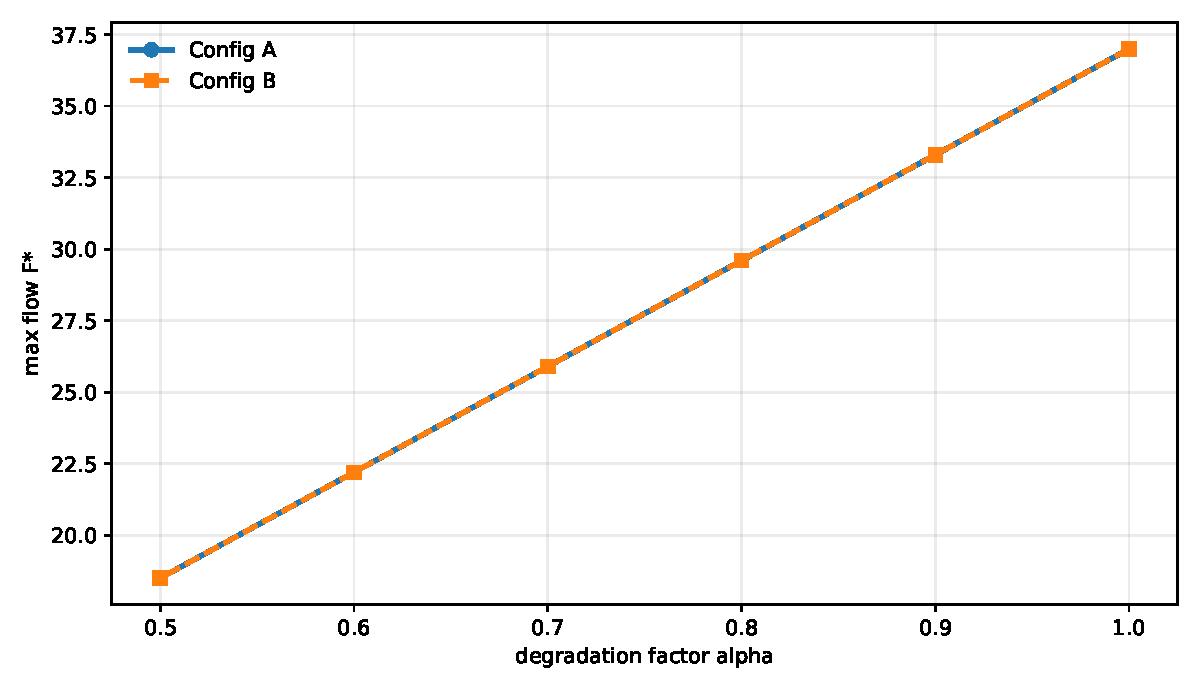
\includegraphics[
  width=0.72\textheight,
  height=0.8\textwidth,
  keepaspectratio
]{degradation_trajectory}
\caption{Degradation trajectory $F^\star(\alpha)$ for Configurations A and B under uniform capacity scaling.}
\label{fig:degradation_trajectory}
\end{figure}

\begin{figure}[ht]
\centering
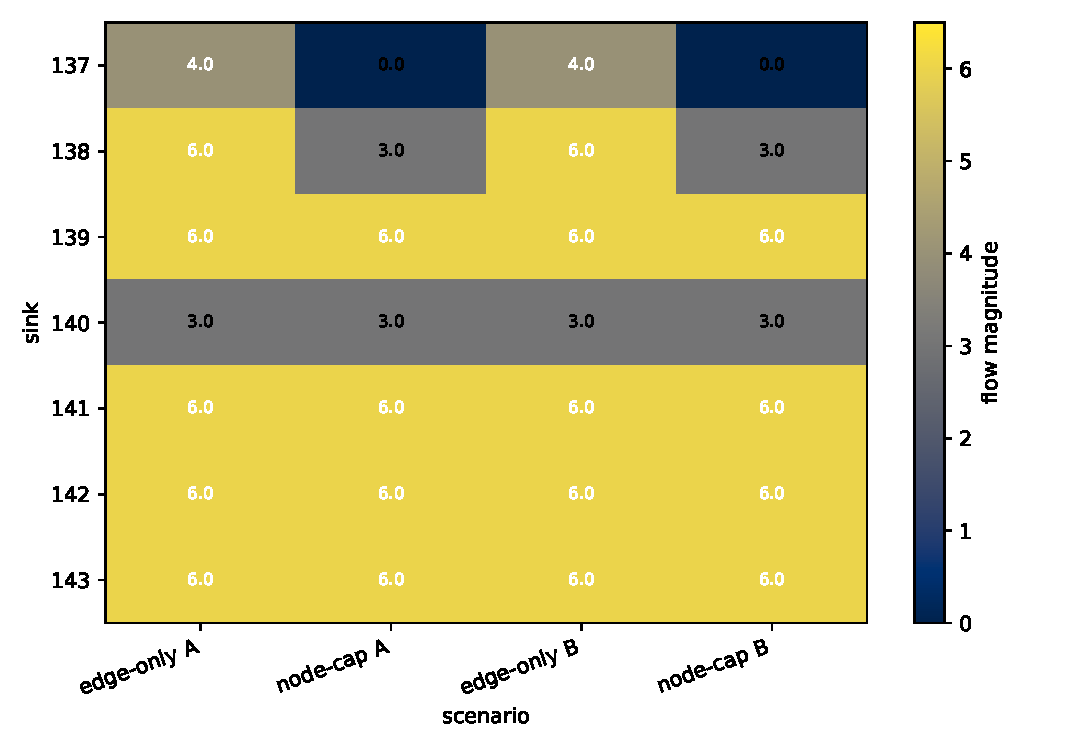
\includegraphics[
  width=0.72\textheight,
  height=0.8\textwidth,
  keepaspectratio
]{sink_flow_heatmap}
\caption{Sink-flow comparison for edge-only and node-capacitated solves across Configurations A and B.}
\label{fig:sink_flow_heatmap}
\end{figure}


\begin{table}[htbp]
\centering
\caption{Min-cut enumeration for Configuration A.}
\label{tab:mincut_enumeration_config_a}
\begin{tabular}{lp{10cm}}
\toprule
Cut & Crossing edges \\
\midrule
1 & $(128\rightarrow134)$, $(128\rightarrow135)$, $(129\rightarrow134)$, $(129\rightarrow135)$, \\
  & $(130\rightarrow134)$, $(130\rightarrow135)$, $(131\rightarrow134)$, $(131\rightarrow135)$, \\
  & $(132\rightarrow134)$, $(132\rightarrow135)$, $(132\rightarrow140)$, $(133\rightarrow134)$, \\
  & $(133\rightarrow135)$ \\
\midrule
2 & $(128\rightarrow135)$, $(129\rightarrow135)$, $(130\rightarrow135)$, $(131\rightarrow135)$, \\
  & $(132\rightarrow135)$, $(132\rightarrow140)$, $(133\rightarrow135)$, $(134\rightarrow136)$ \\
\midrule
3 & $(128\rightarrow134)$, $(129\rightarrow134)$, $(130\rightarrow134)$, $(131\rightarrow134)$, \\
  & $(132\rightarrow134)$, $(132\rightarrow140)$, $(133\rightarrow134)$, $(135\rightarrow136)$ \\
\midrule
4 & $(132\rightarrow140)$, $(134\rightarrow136)$, $(135\rightarrow136)$ \\
\bottomrule
\end{tabular}
\end{table}

\clearpage

% Standalone-only bibliography. Under the thesis build (\maindoc) the whole document shares
% one biblatex bibliography from ../../references.bib, which already carries ford1956,
% ford1962 and birnbaum1969 (the only keys this chapter cites).


\subsection{The IEEE Reliability Test System}
\label{sec:flow-rts24}

The case study is the 24-bus IEEE Reliability Test System \cite{ieee1979rts,grigg1999rts},
taken from the MATPOWER case file \texttt{case24\_ieee\_rts} \cite{zimmerman2011matpower}. The
system has 24 buses, 33 generating units at eleven buses with a total nameplate capacity of
3405~MW, 38 transmission lines of which four are double-circuit pairs, and a peak demand of
2850~MW at seventeen buses. Line ratings in MVA are the edge capacities and generator
nameplate capacities are the node capacities. The physical network is meshed, and the graph
object of Chapter~\ref{ch:system-model} requires a DAG, so each line was oriented by the
direction of its real-power flow in a DC power flow at peak load, with generation dispatched
at a uniform participation factor so that total generation equals total demand and bus 13 as
the slack bus. Twenty-one of the 34 lines carry flow against the order in which the file lists
their end buses. The four double-circuit pairs, which carry equal flow because their
parameters are identical, become one edge each with the summed rating. No directed cycle
remained after orientation, so no line was dropped. The result is a 24-node, 34-edge DAG
(Figure~\ref{fig:flow-rts24}) whose zero-in-degree nodes (buses 7, 21, 22 and 23) are exactly
the buses with generation and no load, and whose zero-out-degree nodes (buses 4, 5, 6, 8 and
19) are exactly the buses with load and no generation, which is consistent with the
orientation being physical. The orientation log and the input files are in
Appendix~\ref{app:network-specs}.

\begin{figure}[htbp]
  \centering
  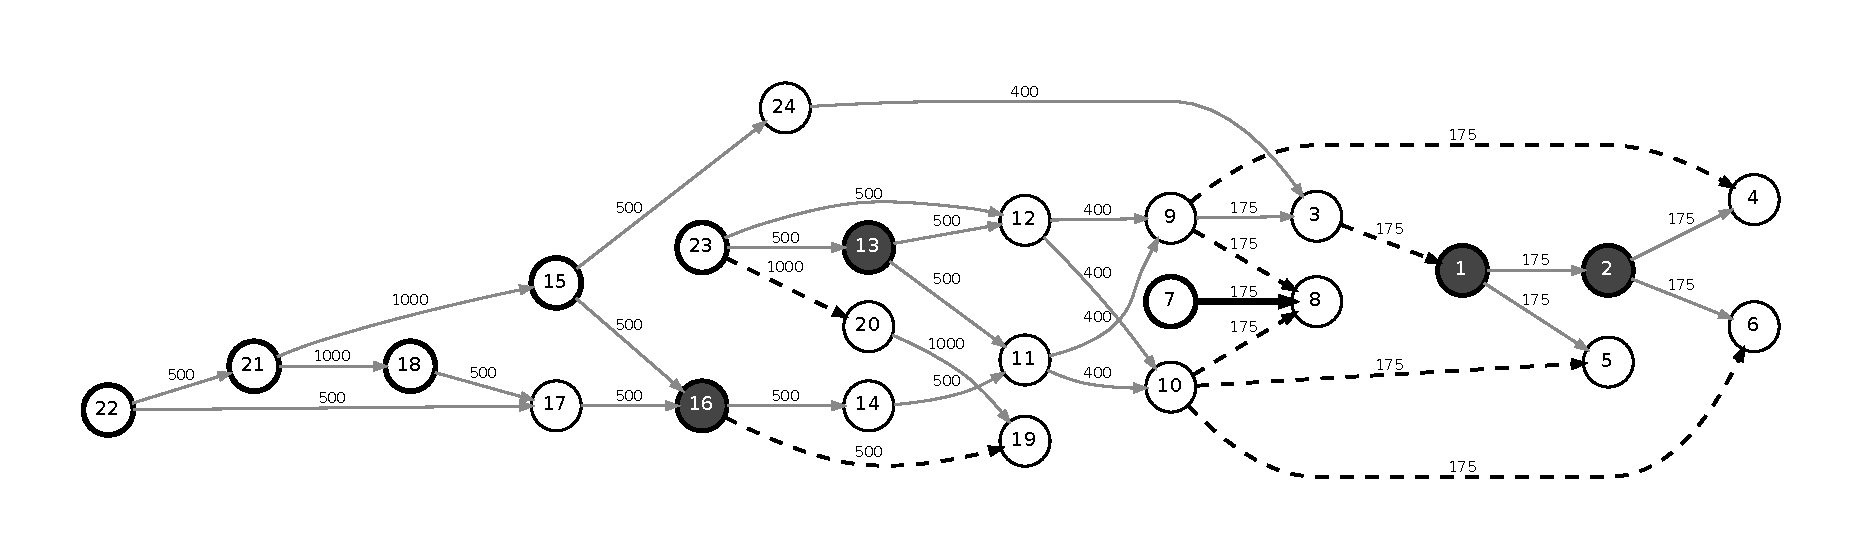
\includegraphics[width=\linewidth]{rts24_dag/rts24_dag.pdf}
  \caption{IEEE RTS-24 oriented by DC power flow at peak load. Edge labels are line ratings
  in MVA; double-circuit pairs are one edge with the summed rating. Bold outlines mark the
  eleven generator buses, and filled nodes mark the four generators (buses 1, 2, 13 and 16)
  that are at their nameplate limit in the maximum flow found under the net-injection
  model. The
  bold line 7--8 has 4~MVA of headroom, the least of any line. Dashed lines form the
  nine-line binding cut of the structural-subset model.}
  \label{fig:flow-rts24}
\end{figure}

Seven buses carry both generation and load and are therefore neither a source nor a sink of
the DAG. To measure deliverable throughput against the whole system demand, a super-source is
connected to every bus whose net injection (generator capacity minus local load) is
positive, with capacity equal to that net injection, and every bus whose net injection is
negative is connected to a super-sink with capacity equal to its net load. A bus with both
generation and load appears once, under its net sign; bus 15, for instance, has 215~MW of
generation and 317~MW of load and is a net importer of 102~MW. The nine net-export buses
offer 2162~MW to the network, the eleven net-import buses require 1607~MW from it, and the
remaining 1243~MW of demand is served locally at export buses without entering the network.

Under this model the delivered throughput equals the net import demand, so the whole of the
system peak demand is met once the load served locally at the export buses is counted. The
same cut binds with generator capacities applied and with generation unconstrained, so at
peak load neither the lines nor the generators limit delivery, and the maximum flow is set
by the demand. No bus is a single point of failure, and the single-line and
single-generator failure rankings are both empty, because every line and every generator has
slack in the flow found. This is a statement about aggregate throughput under a flow model.
Operational security is a separate question, since a remaining path could overload under a
redispatch that the model does not represent. The minimum cut is unique: the lattice of
Section~\ref{sec:flow-mincut} has an empty free zone and the enumeration is complete, and no
generator edge lies in it. Table~\ref{tab:flow-rts24} collects the figures. Should demand
grow, the system would bind first at the four generators already sitting at their nameplate
limit and at the one line with a few MVA of headroom.

For contrast, the first analysis of the same DAG took only the four generation-only buses as
sources and the five load-only buses as sinks, ignoring the mixed buses. Under that model the
network delivers 2725~MVA with edge capacities alone and 1135~MVA with generator capacities,
the binding cut is the nine dashed lines of Figure~\ref{fig:flow-rts24}, and the most damaging
single-line failures are the two double circuits at bus 20 (1000~MVA each), line 16--19
(500~MVA) and lines 3--1 and 7--8 (175~MVA each). The two models answer different questions,
and the difference between them is the reason the net-injection model is the one reported:
the structural-subset model measures a transmission bottleneck that appears only when the
mixed buses are excluded from supply and demand, and those buses do not exist as pure
sources and sinks in the real system.

\begin{table}[htbp]
\centering
\caption{IEEE RTS-24 under the net-injection model at peak load.}
\label{tab:flow-rts24}
\small
\renewcommand{\arraystretch}{1.15}
\begin{tabular}{ll}
\toprule
Quantity & Value \\
\midrule
System peak demand & 2850~MW \\
Demand served locally at export buses & 1243~MW \\
Net import demand & 1607~MW \\
Deliverable throughput, generator capacities applied & 1607~MW (100 per cent) \\
Deliverable throughput, generation unconstrained & 1607~MW \\
Binding cut & the eleven import-bus edges, 1607~MW \\
Single points of failure & none \\
Single-line failures reducing throughput & none \\
Single-generator failures reducing throughput & none \\
Generators at nameplate limit in the flow found & buses 1, 2, 13, 16 \\
Line with least headroom & 7--8, 171 of 175~MVA \\
\bottomrule
\end{tabular}
\end{table}

\subsection{Scale}
\label{sec:flow-scale}

The solvers were timed on four generated instances of the \texttt{genrmf} mesh family used in
the DIMACS implementation challenge \cite{johnson1993dimacs}. The generator here produces the
same layered mesh topology with every edge directed forward, so that the instances are DAGs,
and they are therefore a variant of the published family and not its output. Sizes are 360
nodes and 924 edges, 3,332 and 9,324, 27,040 and 78,364, and 36,992 and 107,644, with
capacities up to 1000 from a recorded seed. Table~\ref{tab:flow-dimacs} gives the warm
second-call times. Dinic is the fastest of the three on every instance and completes the
largest in under a second; push-relabel is within a factor of four; Edmonds-Karp was not run
above 50,000 edges, where its $O(VE^2)$ bound makes it impractical. The external oracle,
which agrees with all three on every instance, takes 29~s on the largest. The comparison is
between implementations on the same machine and says nothing about the algorithms in
general; it establishes that the toolkit's default solver handles networks two orders of
magnitude larger than any in the corpus in interactive time.

\begin{table}[htbp]
\centering
\caption{Warm second-call solve times on DAG variants of the \texttt{genrmf} mesh family.
Edmonds-Karp was not run above 50,000 edges.}
\label{tab:flow-dimacs}
\small
\renewcommand{\arraystretch}{1.15}
\begin{tabular}{lrrrrr}
\toprule
Instance & Nodes & Edges & Dinic (s) & Push-relabel (s) & Edmonds-Karp (s) \\
\midrule
small  & 360    & 924     & 0.002 & 0.097 & 0.007 \\
medium & 3,332  & 9,324   & 0.017 & 0.019 & 0.179 \\
large  & 27,040 & 78,364  & 0.961 & 1.520 & -- \\
xlarge & 36,992 & 107,644 & 0.657 & 2.277 & -- \\
\bottomrule
\end{tabular}
\end{table}

\section{Discussion}
\label{sec:flow-discussion}

The toolkit is point-valued. An interval or probability-box capacity is not propagated, and
running the best-case and worst-case capacities gives two solves whose relation to the true
range of the maximum flow is a bound only because the maximum flow is monotone in every
capacity. Extending the toolkit to intervals by that monotonicity argument is direct for the
flow value; the cut structure, the failure rankings and the thresholds are not monotone and
would need the same kind of treatment that the floats received in
Chapter~\ref{ch:critical-path}.

Exactness in this chapter is on the evaluated candidates. The sensitivity and failure modules
restrict their candidates to the saturated edges and to the edges of some minimum cut, and
their results are exact on those sets. An edge outside the candidate set cannot change the
maximum flow by a small change in its capacity, but a large enough change can, and the
$k$-edge failure analysis is exhaustive only over the candidate set.

The toolkit computes no probability. It does not answer the stochastic-flow question of
Chapter~\ref{ch:lit-review}, the probability that a stated demand can be met, and it does not
weight a failure by its likelihood. That combination is a natural extension, since the
probability toolkit of Chapter~\ref{ch:probability-toolkit} gives the probability that a
component operates, but it is not built.

All analyses are on a single fixed-capacity instance. Time-varying degradation and adaptive
rerouting are outside the model, and the degradation scenarios of
Section~\ref{sec:flow-failure} are a sequence of separate instances.

The global edge and node connectivity of a DAG, defined as the minimum over all ordered node
pairs of the unit-capacity maximum flow, is zero, because a sink has no outgoing edge and
every DAG has a sink. The implementation computed exactly that definition and therefore
returned zero on every network, which the validation confirmed independently. The
whole-graph definition is the one the module documents and computes, and it is left as it
is. The quantity that answers the redundancy question on a DAG is the minimum over declared
source and sink pairs, which the per-pair disjoint-path counts of
Section~\ref{sec:flow-structure} already give; a named metric for that minimum is listed in
Chapter~\ref{ch:conclusions}.

Two further extensions follow from the model. Minimum-cost flow, in which each edge carries a
cost per unit as well as a capacity, would answer how a given demand is met most cheaply, and
a time-expanded network would carry the flow model across a planning horizon. Both are listed
in Chapter~\ref{ch:conclusions}.

\section{Summary}
\label{sec:flow-summary}

The Capacity Flow Toolkit answers six questions about a capacitated DAG. The flow model has
been stated, with the reductions for several sources and sinks and for node
capacities proved exact, and three maximum-flow solvers have been provided on the graph
object of Chapter~\ref{ch:system-model}, each result checked for feasibility, conservation
and agreement between flow and cut. Six questions have been answered by modules that share
one baseline solve: throughput and margin, the binding cut and the lattice of every
equivalent cut, the most damaging failures and degradations, the marginal value and range of
each edge, degradation and upgrade thresholds by a partition-change search, and redundancy
and single points of failure. The toolkit has been validated against an external oracle and
brute-force enumeration on twelve networks, timed on generated instances of up to $10^5$
edges, and applied to the IEEE Reliability Test System, on which neither lines nor generators
bind at peak load and the nearest constraints are four generators and one line. The toolkit is point-valued, and its extension to interval
capacities and to probability-weighted measures is left to future work.

\ifdefined\maindoc
% do nothing
\else
\printbibliography
\end{document}
\fi